\chapter{Mechanisms Controlling the Land/Sea Contrast} 

\tableofcontents % Write out the Table of Contents

\label{mechanisms} 

\lhead{Chapter 4. \emph{Mechanisms}} 

\section{Introduction}
% \paragraph{Discuss GW theories, relevance to interannual var.}
In chapter \ref{evidence} we showed evidence for the interannual land/ocean 
temperature contrast in observations and models, and discussed its magnitude and 
spatial extent. Through AMIP simulations it was shown that an $R_{l/o}>1$ can 
exist in a model forced only with SST variability. The implication is that the 
variability from the ocean is being amplified over the continents. By 
prescribing SSTs we remove the effect of ocean heat capacity - and it's ability 
to cause $R_{l/o}>1$ by damping the ocean's response relative to the land 
response for a uniform forcing. In this chapter we will attempt to determine the 
underlying mechanisms responsible for the amplification of ocean surface 
temperature anomalies over land. A range of sensitivity experiments using the 
ACCESS, MIT RCE and GREB models will be presented.  The analysis of observations 
and models from chapter \ref{evidence} also demonstrated that the ability of the 
ocean to influence land temperatures is geographically inhomogenous. There is a  
latitudinal dependence, and this will guide the initial investigations of this 
chapter.

%----------------------------------------------------------------------------------------
%	influence of SSTs on Continental temps
%----------------------------------------------------------------------------------------

\section{The Influence of Tropical Oceans on Land}

When looking at the relationship between $T_{land}$ and SSTs there is an 
assymetry between the response of $T_{land}$ to tropical and extra-tropical SST 
forcing. We investigate this assymetry and the importance of the tropical oceans 
in regulating regional and global land surface temperatures using modelling 
experiments. In the 1K experiments a constant +/-1K SST anomaly is applied to 
tropical or extra-tropical regions, in the Half-AMIP experiments the same 
regional restrictions are used but instead of a constant forcing, variability is 
imposed using observed SST anomalies. The Pacemaker experiments are forced with 
an idealised ENSO in the tropical Pacific and a slab ocean or fixed SSTs 
elsewhere.

\subsection{1K Experiments}

Figure \ref{fig:1K} shows the surface temperature response (control removed) 
from the 1K experiments; where 1K was added to the oceans in the tropics, 
extra-tropics or globally. In response to a tropical SST perturbation there is a 
large tropical response, greatest over equatorial South America and Africa, 
India and the maritime continent (Fig.\ref{fig:1K} a). The tropical 1K ocean 
perturbation leads to $T_{land}>+1$K in most tropical areas. Thus the SST 
forcing is amplified. The extra-tropical land the response to the tropical 
forcing is not significant everywhere, but some regions also show an amplified 
response to the tropical SST forcing (e.g. central Asia and parts of Europe and 
North America).  An extra-tropical $T_{land}$ response to tropical SSTs is seen 
for seasonal averages in the winter months of each hemisphere, the Northen 
Hemsiphere winter response is shown in Figure \ref{fig:1K} e.

When looking at the annual mean response of $T_{land}$ to extra-tropical SST 
perturbations there is little significant response, however for seasonal 
averages both hemispheres show a significant response in their respective winter 
months, shown for the Northern Hemisphere in Figure \ref{fig:1K} e-g. The 
response of $T_{land}$ is also amplified in some regions relative to the initial 
perturbation.  However, the extra-tropical forcing again leads to a weaker land 
response than the tropical forcing, as was also found in the AMIP simulations.  
Also similar to the AMIP simulations we again find that the  global SST forcing 
has a bigger impact than the tropical only forcing for the annual mean. In 
addition the response of the global SST forcing is greater than the 
superposition of the tropical and extra-tropical forcing (comparing 
Fig.\ref{fig:1K} c and d).  This again indirectly suggests that the 
extra-tropical SST forcing does lead to a significant land response.

\begin{figure}[ht]
	\centering
	\includegraphics[width=0.45\textwidth]{{meantemp.trop}.eps}
	\includegraphics[width=0.45\textwidth]{{meantemp.trop.DJF}.eps}\\
\vspace{-0.9cm}
	\includegraphics[width=0.45\textwidth]{{meantemp.extr}.eps}
	\includegraphics[width=0.45\textwidth]{{meantemp.extr.DJF}.eps}\\
\vspace{-0.9cm}
	\includegraphics[width=0.45\textwidth]{{meantemp.glob}.eps}
	\includegraphics[width=0.45\textwidth]{{meantemp.glob.DJF}.eps}\\
\vspace{-0.5cm}
	\includegraphics[width=0.45\textwidth]{{meantemp.addt}.eps}
	\includegraphics[width=0.45\textwidth]{{meantemp.addt.DJF}.eps}\\
\caption{Mean $T_{surf}$ response for sensitivity experiments  a) 1K added to 
	tropical oceans b) 1K added to extra-tropical oceans c) 1K added to global 
	oceans d) Combined response of tropical 1K oceans plus extra-tropical 1K 
	ocean. Masked at 95\% confidence levels.}
\label{fig:1K}
\end{figure}



\subsection{Half-AMIP Experiments}

In Figure \ref{fig:ftest} f-tests are used to measure the increase in annual 
temperature variability due to SST variability at the surface and at the 300hPa 
pressure level relative to a simulation with fixed SST climatology. Figure  
\ref{fig:ftest} a) and d) show that global SST variability has a substantial 
impact on the tropical atmospheric and surface temperature variability. In the 
extra-tropical regions the impact is much weaker, but still statistically 
significant in some regions.

In order to separate the influence of the tropical SST variability from that of 
the extra-tropical SST, we repeat the AMIP experiment forced with the historical 
SST variability just in the tropics or just in the extra-tropical regions. The 
impact of the tropical-only SST variability is similar to the global SST 
variability, with a clear and strong impact in the tropical regions.  The AMIP 
simulation with extra-tropical-only SST variability has only a very weak to no 
impact on the regional (grid-box scale) atmospheric and surface temperature 
variability.  However, if we compare the global AMIP versus the tropical only 
AMIP run we still can see a somewhat larger increase in variance over land in 
the global AMIP run. This indirectly suggests that the extra-tropical SST 
forcing does play a role, although it is much smaller than the tropical forcing.  
In summary the AMIP experiments suggest a clear tropical SST forcing to the 
atmospheric and land surface temperatures, but a much weaker or no forcing from 
the extra-tropical SST.

\begin{figure}[ht]
	\includegraphics[width=1.0\textwidth, trim={8.5cm 5cm 11cm 
	1cm},clip=true]{{ftest_sub_sfc}.pdf}
	%\vspace{-1.8cm}
	\includegraphics[width=1.0\textwidth, trim={8.5cm 5cm 11cm 
	1cm},clip=true]{{ftest_sub_300}.pdf}
	\caption{F-test of annual mean temperature for AMIP-type runs. Surface 
		temperature response on top row, 300hPa response on bottom row.	a),d) AMIP 
		run with detrended HadISST used globally b),e) AMIP-type run with detrended 
		HadISST in extra-tropics, climatological SSTs elsewhere c),f) AMIP-type run 
		with detrended HadISST in tropics, climatological SSTs elsewhere tropics.  
		All values masked at 90\% confidence levels. Hatching indicates areas of 
	ocean with SST variability.}
	\label{fig:ftest}
\end{figure}

\subsection{Tropical Troposphere}
The Half-AMIP experiments demonstrate an important process in the strong 
tropical land/ocean connection. Figures \ref{fig:ftest} d)--e) show the value of 
an f-test on the 300hPa surface, measuring the increase (values above zero) in 
temperature variability due to imposed SST variability. The results for global 
and tropical AMIP runs are very similar, with the global AMIP having slightly 
higher values in the tropics and some more variability in the extratropics, 
whereas there's no significant tropospheric response to extra-tropical SSTs.  
The tropospheric response in the tropics can be described with two key 
processes; the large amplitude of the temperature variability is due to latent 
heating by deep moist convection, and the -- largely -- zonally uniform pattern 
is the result of the tropical free troposphere not being able to maintain 
horizontal pressure gradients due the small coriolis number (REF). This results 
in tropical SST perturbations being amplified in the troposphere and efficiently 
transported over tropical land. The area with the largest tropospheric anomalies 
is over the eastern tropical pacific, the ENSO region. ENSO is the dominant 
driver of interannual temperature variability and while the ENSO induced 
tropospheric anomalies are distributed around the tropics, there is still a 
maximum in that area. The role of ENSO is further explored with the Pacemaker 
experiments.


%----------------------------------------------------------------------------------------
%	ENSO
%----------------------------------------------------------------------------------------

\subsection{Pacemaker Experiments}\label{pacemaker}

On inter-annual timescales ENSO is the most significant global climate driver. 
It is therefore remarkable that in the analysis of the CMIP5 model simulations 
the NINO3 region did not show up with a high correlation to global $T_{land}$ 
(see Fig.\ref{fig:cmip_cormap}). The ENSO region in the tropical Pacific has a 
lower correlation with $T_{land}$ than adjacent regions and the other ocean 
basins. Using the combined monthly mean CMIP5 surface temperature anomalies, 
Fig.\ref{fig:xcor} e) shows the lagged correlations between NINO3 SST and global 
$T_{land}$. The NINO3 region is seen to lead global land by 4 months.  Typically 
land has a fast response time to forcings, which would not result in a 
4 month delay, so this result suggests that the full land response is not 
directly forced by the NINO3 SST but is most likely caused by something else. 
This other forcing may be delayed to the ENSO variability by about 4 months. 
Since we have seen in Fig.\ref{fig:cmip_cormap} that global $T_{land}$ is highly 
correlated to other tropical ocean SST, it seems likely that $T_{land}$ is 
linked to the slower ocean response in the remote tropical oceans and not 
directly to the NINO3 region.

To address this question we conducted a series of idealised ENSO-response 
experiments. In the first experiment we prescribe an oscillating ENSO pattern (a 
regression between NINO3 and SSTs shown in Fig.\ref{fig:regpat}) in the tropical 
Pacific and a fixed 12 month climatology of SSTs elsewhere.  The oscillation 
period of the ENSO signal is 4 years, peaking in January. In the second 
experiment we allow SST variability outside the tropical Pacific simulated by a 
simple slab ocean model with a mixed layer depth of 50 metres.  Thus, in the 
second experiment the global ocean SSTs can respond to the oscillating ENSO 
pattern forcing.

\begin{figure}[ht]
	\includegraphics[width=\textwidth]{{regpat}.eps}\\
	\caption{Pattern used in ENSO experiments. Result of regression between NINO3 
	and global SST.}
	\label{fig:regpat}
\end{figure}

\subsection{Delayed Response}
Figure \ref{fig:xcor} (i-l) shows cross-correlations from the ENSO-FIXSST and 
ENSO-Slab forcing experiments. In i) and j) we see that for the fixed SST 
experiment the global and tropical land responds to the ENSO-like forcing (red 
line), and does so without the delay seen in Figure \ref{fig:xcor} e). When a 
slab ocean is introduced the land responds with a realistic delay of around 4 
months.  The peak slab ocean response is at 6 months, implying that the land is 
responding immediately to the initial Pacific ocean forcing and then 
subsequently to the delayed slab ocean response. The delayed land response is 
also associated with a higher correlation to the NINO3 region. Comparing the 
global and tropical averages, the main difference is the magnitude of the peak 
correlation, but in the tropics the slab ocean also results in the peak land 
correlation being higher than the peak ocean correlation. So the delayed 
response of the remote tropical oceans to a Pacific ocean forcing explains both 
the delayed land response and some part of the amplification of the oceanic 
temperature signal over land. In the extra-tropics there is only a very weak 
influence of the ENSO forcing on land temperatures in the sensitivity 
experiments (Fig.  \ref{fig:xcor} g, h), and the tropical Pacific has little 
influence on the slab ocean in the extra-tropics. The observations and CMIP5 
models also don't show a significant relationship between the extra-tropics and 
NINO3 (Fig.\ref{fig:xcor} g,h,k,l).

\clearpage
\begin{figure}[ht]
	\includegraphics[width=\textwidth, trim={5cm -1cm 5cm 
	-0.5cm},clip=true]{{xcor_sub_obs}.eps}
	\includegraphics[width=\textwidth, trim={5cm -1cm 5cm 
	-0.5cm},clip=true]{{xcor_sub_cmip5}.eps}
	\includegraphics[width=\textwidth, trim={5cm -1cm 5cm 
	-0.5cm},clip=true]{{xcor_sub_enso}.eps}
\caption{Cross-correlations between the NINO3 region and land and ocean.  
	Observations (top row), combined CMIP5 models (middle row), Two sensitivity 
	experiments (bottom row);  Atmospheric model forced with ENSO-like oscillation 
	in tropical Pacific and fixed SSTs elsewhere (red line), slab ocean elsewhere 
	(green, blue lines).  Global land and ocean (a,e,i), tropical land and ocean 
	(b,f,j), NH extra-tropical land and ocean (c,g,k) and SH extra-tropical land 
	and ocean (d,h,l).  NINO3 autocorrelation included for reference (black dashed 
line).}
	\label{fig:xcor}
\end{figure}



To summarise thus far; we see that tropical SSTs strongly influence tropical and 
- to a lesser extent - extra-tropical continental temperatures; SST anomalies 
are amplified in the tropical troposphere and efficiently transported over land; 
ENSO is the dominant source of interannual variability and can influence land 
surface temperatures via the troposphere. However we now wish to investigate the 
process by which SST variability leads to amplified $T_{land}$ variability.  

% \section{ENSO}
% \begin{itemize}
% 	\item ENSO is source of tropical inter-annual variability.
% 	\item Temperature anomaly seen throughout tropical troposphere
% 	\item Land responds quickly - within a month - to initial anomaly.
% 	\item Remote tropical oceans response is delayed by 3-4 months.
% 	\item Timing of delay of remote tropical oceans is a function of mixed layer 
% 		depth.
% 	\item Land responds to the delayed forcing by remote trop oceans.
% 	\item Mean land response appears to be delayed, i.e. when plotted with lag 
% 		correlations.
% 	\item Delayed land response is linear combination of initial response to 
% 		Pacific ocean and response to delayed remote tropical oceans.
% 	\item Land response is amplified due to previously discussed process.
% 	\item The land response is further amplified by secondary response to remote 
% 		tropics.
% \end{itemize}


%----------------------------------------------------------------------------------------
%	LAPSE RATE
%----------------------------------------------------------------------------------------

\section{The Lapse Rate Mechanism}

We are now going to investigate the relationship between tropospheric anomalies 
and the surface by looking at the warming lapse rate mechanism described by 
\citet{Joshi2007} and \citet{Byrne2013a}, and testing it's validity for 
interannual variability. 

We first take a look at the vertical structure of the relationship between land 
and ocean temperatures comparing the Pacemaker experiment with a climatology run 
(i.e. no SST variability).  Using tropical averages, Figure 
\ref{fig:linreg_plev} shows regression values for the $T_{tropos}$ at different 
pressure levels as a function of the surface temperature $T_{land}$ (a) and 
$T_{ocean}$ (b), with the green line for the column of air above tropical land, 
blue for the column of air above tropical ocean, and the black line is the 
column above the remote tropical ocean, essentially the tropical oceans with the 
area of forcing removed.  Looking first at Figure \ref{fig:linreg_plev} a), in 
the simulation without any SST variability (dashed lines) the higher level 
tropical temperatures over land areas are not related to $T_{land}$ as the 
regression values between the surface and tropospheric temperatures falls to 
zero above \SI{800}{\hecto\pascal}, indicating that the atmospheric internal 
$T_{land}$ variability (independent of SST variability) is limited to the near 
surface layers and is not strongly related to the upper free $T_{tropos}$. In 
the simulation with SST variability the tropospheric temperature shows a strong 
relationship with the surface $T_{land}$ variability at all levels. 

Now focusing on Figure \ref{fig:linreg_plev} b), a distinctive feature for the 
troposphere above oceans (blue line) is the large increase in the regression 
values in the upper troposphere. This is a well known signature of moist
convection; a \SI{1}{\kelvin} anomaly at the surface corresponds to a 
\SI{2}{\kelvin} anomaly in the upper level temperatures, due to the latent heat 
release by moist convection (\citet{Joshi2007}, \citet{Byrne2013}, 
\citet{Dommenget2009}, etc.). The anomalies above land regions don't reach the 
same peak in the upper troposphere, however in the middle troposphere, around 
the \SI{700}{\hecto\pascal} to \SI{500}{\hecto\pascal} level, the two lines 
coincide, similar to the level in the atmosphere described by \citet{Joshi2007} 
where there is no land/ocean warming contrast. It's in the levels below 
\SI{800}{\hecto\pascal} where the variability increases above land. This figure 
would indicate a value of $R_{l/o}$ of around 1.2, as for a \SI{1}{\kelvin} 
anomaly of $T_{ocean}$ we have a \SI{1.2}{\kelvin} response in $T_{land}$.  

As we saw in section \ref{pacemaker} the remote oceans are important in the 
timing and magnitude of the continental land ENSO response, so we will now 
discuss their response to the Pacific ocean forcing. An advantage of the 
Pacemaker experimental design is that the area of ocean forcing is very well 
constrained.  In contrast, when using observations or coupled models to look at 
the response to an ENSO forcing the remote tropical oceans will also have their 
own, potentially considerable, internal variabiltiy due to ocean dynamics.  In 
the Pacemaker experiment the remote slab oceans have no dynamics or internal 
variability.  Therefore, we can consider the Pacific Ocean an external forcing 
to both the continental regions and the remote oceans, and measure the seperate 
response of land and ocean.  In Figure \ref{fig:linreg_plev} b) the black line 
is a measurement of the atmospheric response above remote oceans, the only 
variability for this region is imposed via the Pacific ocean forcing.  The 
remote tropical response is similar to the land response in shape; it also lacks 
the large amplification in the upper troposphere indicating that the upper 
levels are responding to the Pacific forcing and not being driven by their own 
moist convection.  At all levels the response above the remote tropical oceans 
is damped when compared to the land response which means there is no clear level 
where there is no land/ocean contrast however the two lines diverge more near 
the surface, with the largest difference between the gradients of the 
temperature profiles below \SI{800}{\hecto\pascal}.  In the global warming lapse 
rate theory, the steeper near-surface continental lapse rate is due to reduced 
moisture availability and thus lower relative humidities. It would appear that a 
similar process is active on interannual timescales with an additional factor; 
the tropospheric profile above a region of the ocean that is responding to an 
external forcing -- or a forcing from a seperate ocean basin -- will be 
potentially be damped throughout the entire troposphere.  The vertical structure 
above land and ocean is further explored with a one and two-dimensional model.
NOTE: further lapse rate analysis on pacemake in 
~/project/pacemaker/figures/*profile*

\begin{figure}[ht]
		\includegraphics[width=0.45\textwidth]{{linreg_land_profile}.eps}
		\includegraphics[width=0.45\textwidth]{{linreg_ocean_sans_profile}.eps}\\
	\caption{Linear regression coefficients for temperature above tropical land 
	and ocean as linear model of a) $T_{land}$ (1000hPa surface) and b) 
$T_{ocean}$, for forced run (solid) and control run (dashed). i.e.  
$T_{plv,land} = a T_{sfc,land} + b$, and $T_{plv,ocean} = a T_{sfc,land} + b$}
\label{fig:linreg_plev}
\end{figure}


\subsection{The Weak Temperature Gradient Approximation}
The Weak Temperature Gradient (WTG) approximation was introduced in 
\ref{intro_wtg}, and it is use in the single column model as a way to parametize 
the large scale circulation. Briefly, the WTG approximation states that as 
temperature gradients ar removed by... If we consider the tropical tropospheric 
temperature to be largely controlled by the ocean surface temperature we can use 
a single column model to study the land/ocean temperature contrast.  Initially a 
range of temperature profiles are generated in an ocean column with varying 
SSTs, then those profile can be imposed above a land surface.  The temperature 
profile is held constant in the free troposphere and allowed to vary near the 
surface, thereby simulating the control of the free tropospheric temperatures by 
(for example) Pacific ocean anomalies.


\subsection{Experiments with a Single-Column Model}
\label{mech_scm}
In order to study the land temperature response to a tropospheric forcing we 
will use a single column model, as it allows us to vary parameters of the land 
surface properties while controlling the tropospheric forcing.  We begin by 
generating the temperature profiles above an ocean column by prescribing a range 
of SSTs and running the model to equilibrium.  The focus of our study is 
interannual variabilty, so we chose an SST value of \SI{26}{\degreeCelsius} as 
the mean profile -- which is appropriate for a tropical profile -- then the SST 
was varied by fractions of a degree above and below the mean value to simulate 
the magnitude of interannual variability. At each value the model was run to 
equilibrium.  In addition to these small SST changes the model was run with 
\SI{1}{\degreeCelsius} increments from \SI{19}{\degreeCelsius} to 
\SI{34}{\degreeCelsius}, to test the response of the model over a wide range of 
SSTs.

The tropospheric response and the amplification of surface anomalies due to 
moist convection is shown in Figure \ref{fig:scmsstprof}.  In 
Fig.\ref{fig:scmsstprof} a) and c) the temperature anomalies relative to the 
mean profile show the amplification with height of both positive and negative 
SST anomalies. Comparing the a) and c) also demonstrates the difference between 
small increment changes in SST (c) -- relative in magnitude to interannual 
variability -- and \SI{1}{\kelvin} increments, and while the former shows much 
greater variation between the profiles the general pattern is still clear, and 
similar to a).  The magnitude is more clearly shown in Fig.\ref{fig:scmsstprof} 
b), which measures the amplification of the SST anomaly with height relative to 
the mean value.  For example, a value of 2 at \SI{300}{\hecto\pascal} indicates 
that a surface anomoly of \SI{1.5}{\kelvin} would lead to a \SI{3}{\kelvin} 
anomaly at that height.  It shows that positive and negative anomalies are 
amplified to a similar extant, although the tropopause is higher for the 
positive anomalies leading to a discrepency around \SI{200}{\hecto\pascal}.  
Figure \ref{fig:scmsstprof} c) demonstrates that the upper tropospheric 
anomalies are a result of heating by moist convection. (Not shown) Plots of the 
heating due to dry convection show uniform heating rate throughout the 
troposphere.

\begin{figure}[ht]
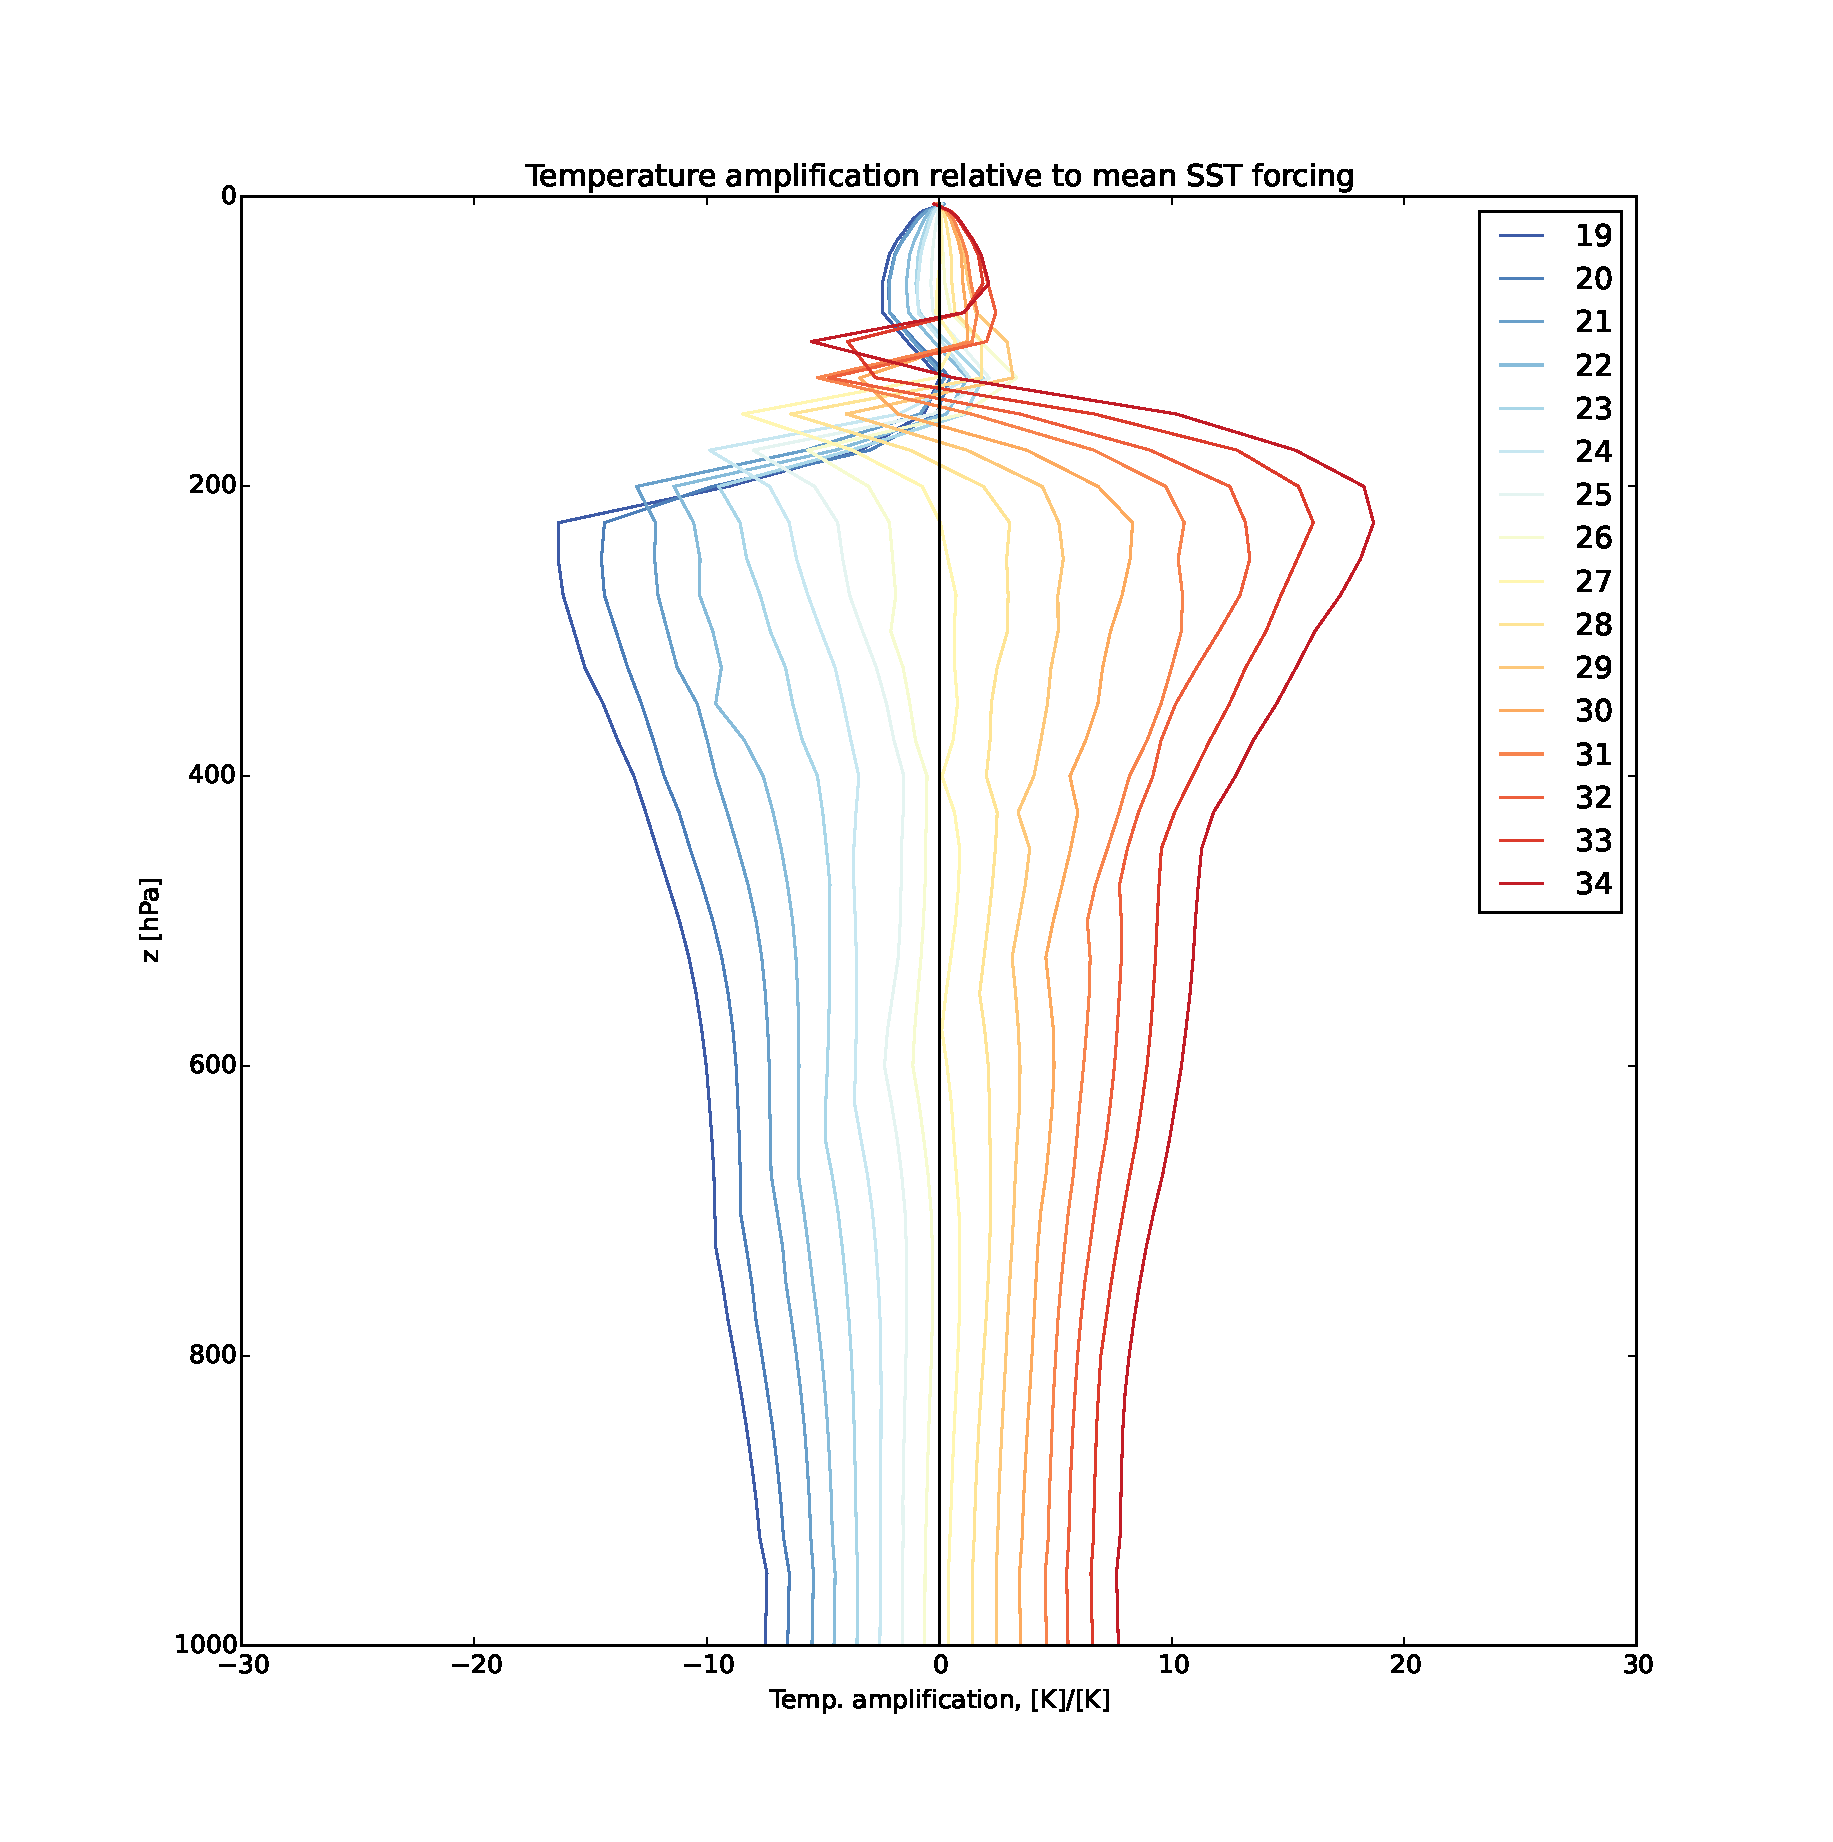
\includegraphics[width=0.5\textwidth]{enso_prof_temp_mean.eps}
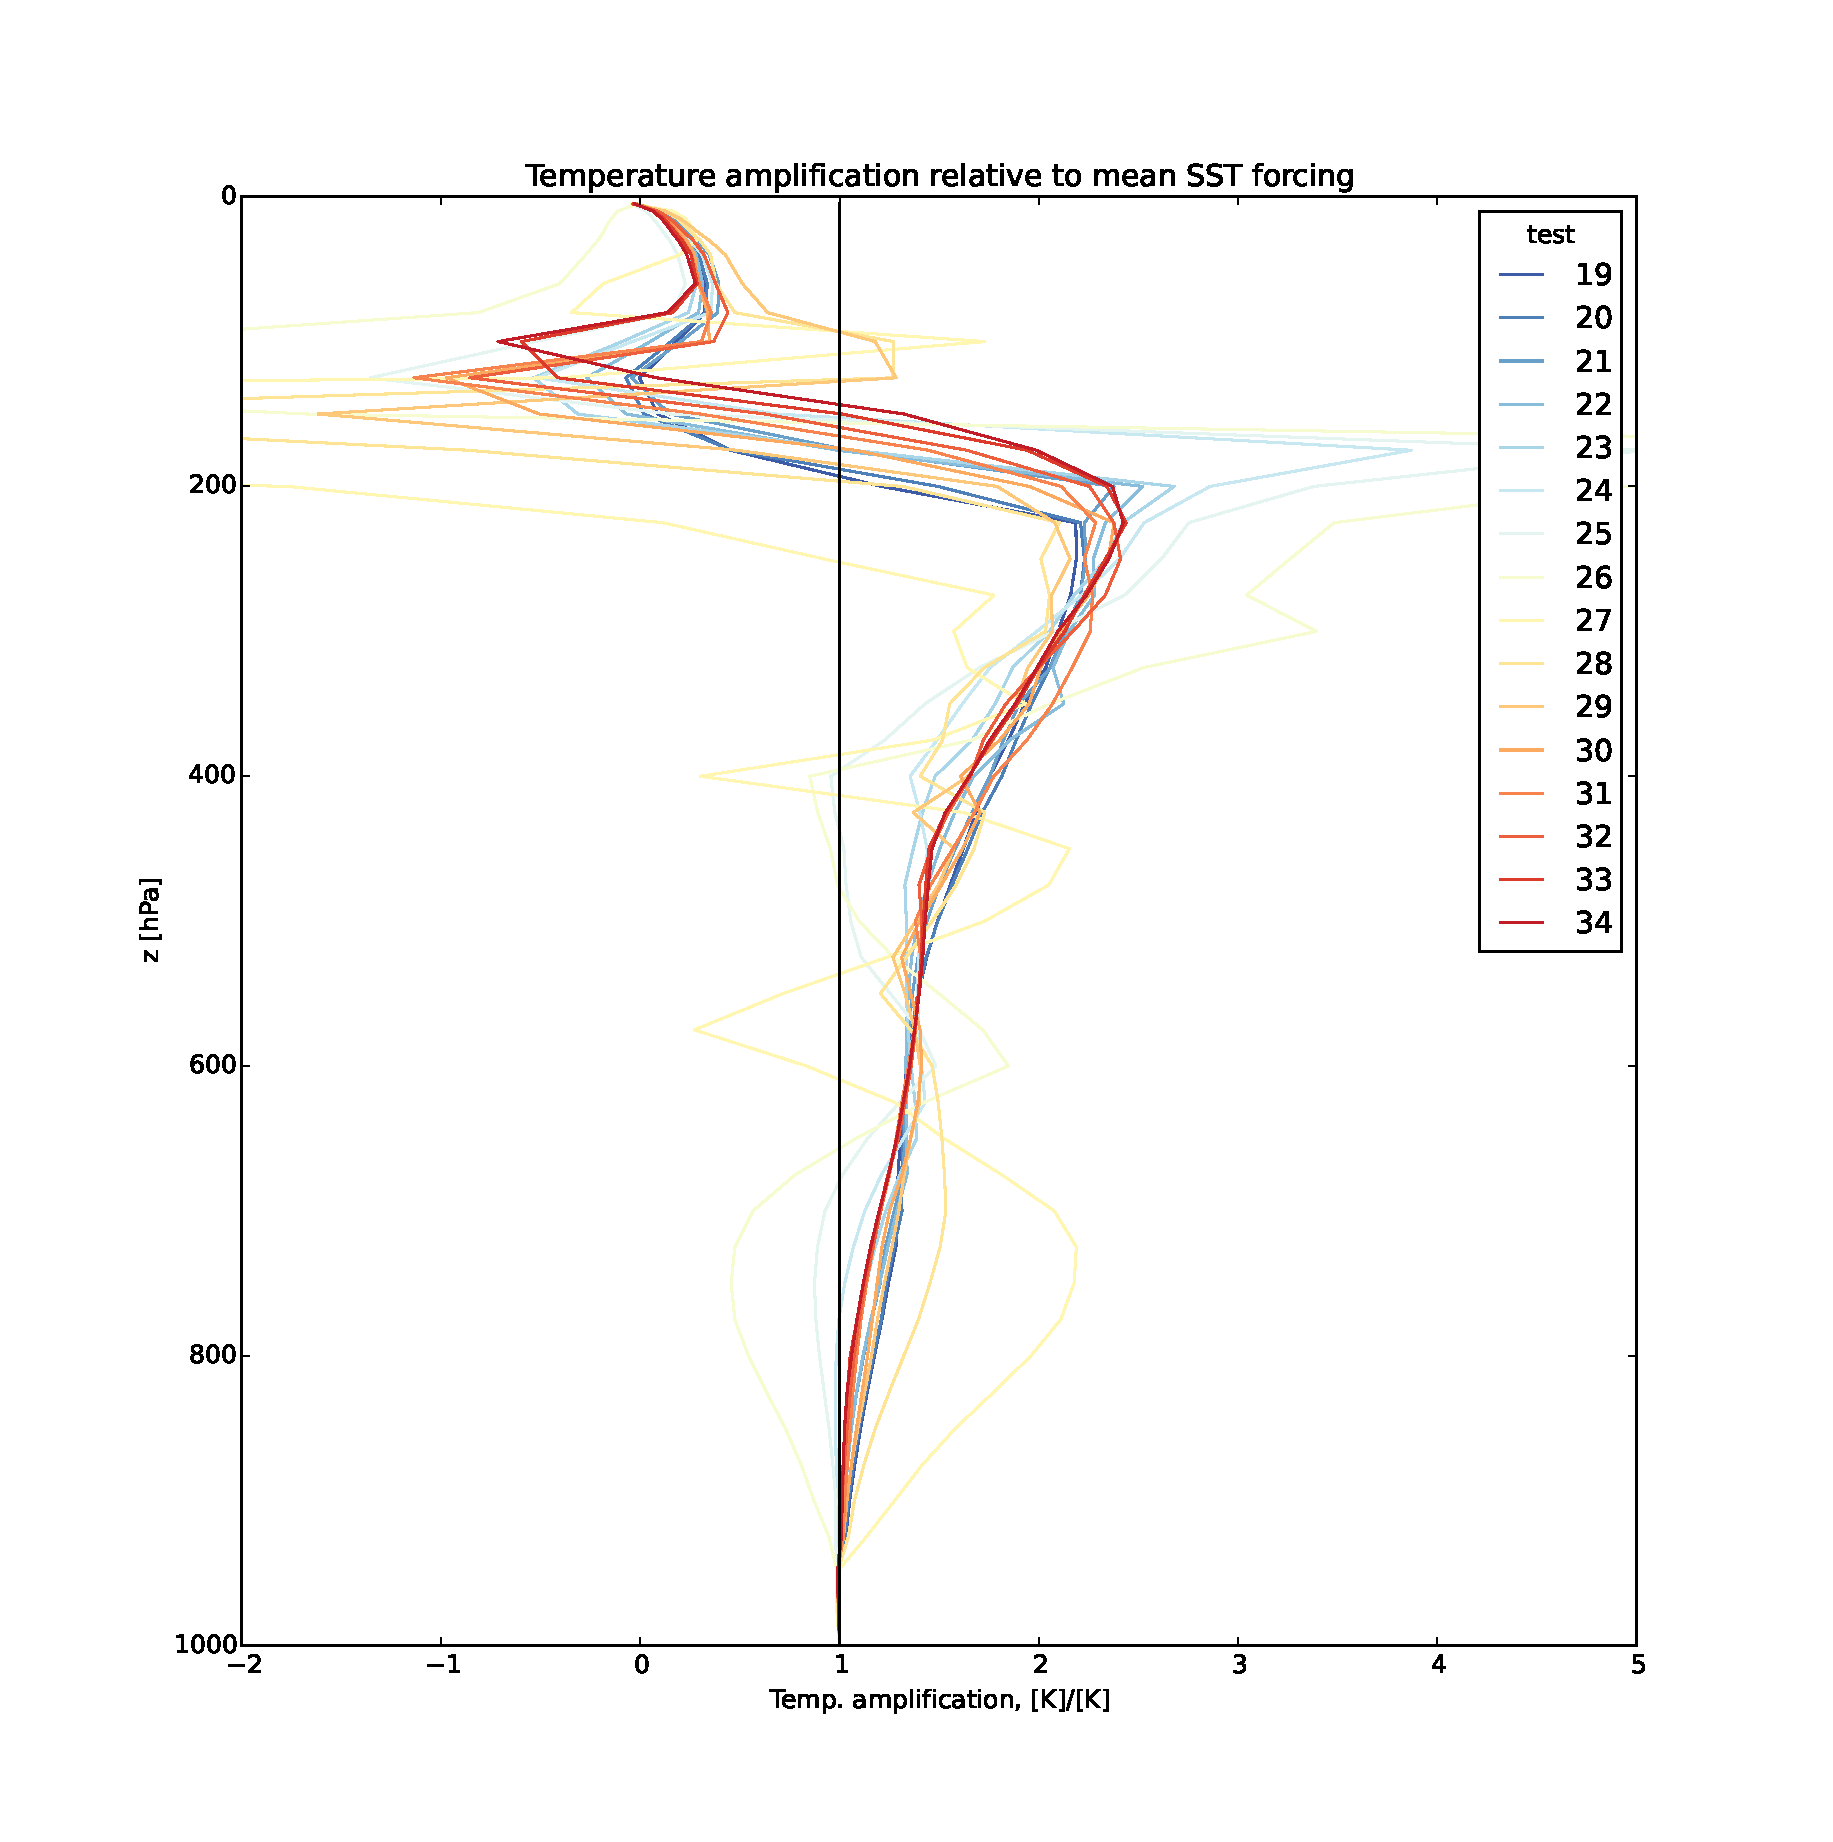
\includegraphics[width=0.5\textwidth]{enso_prof_ampratio_mean.eps}\\
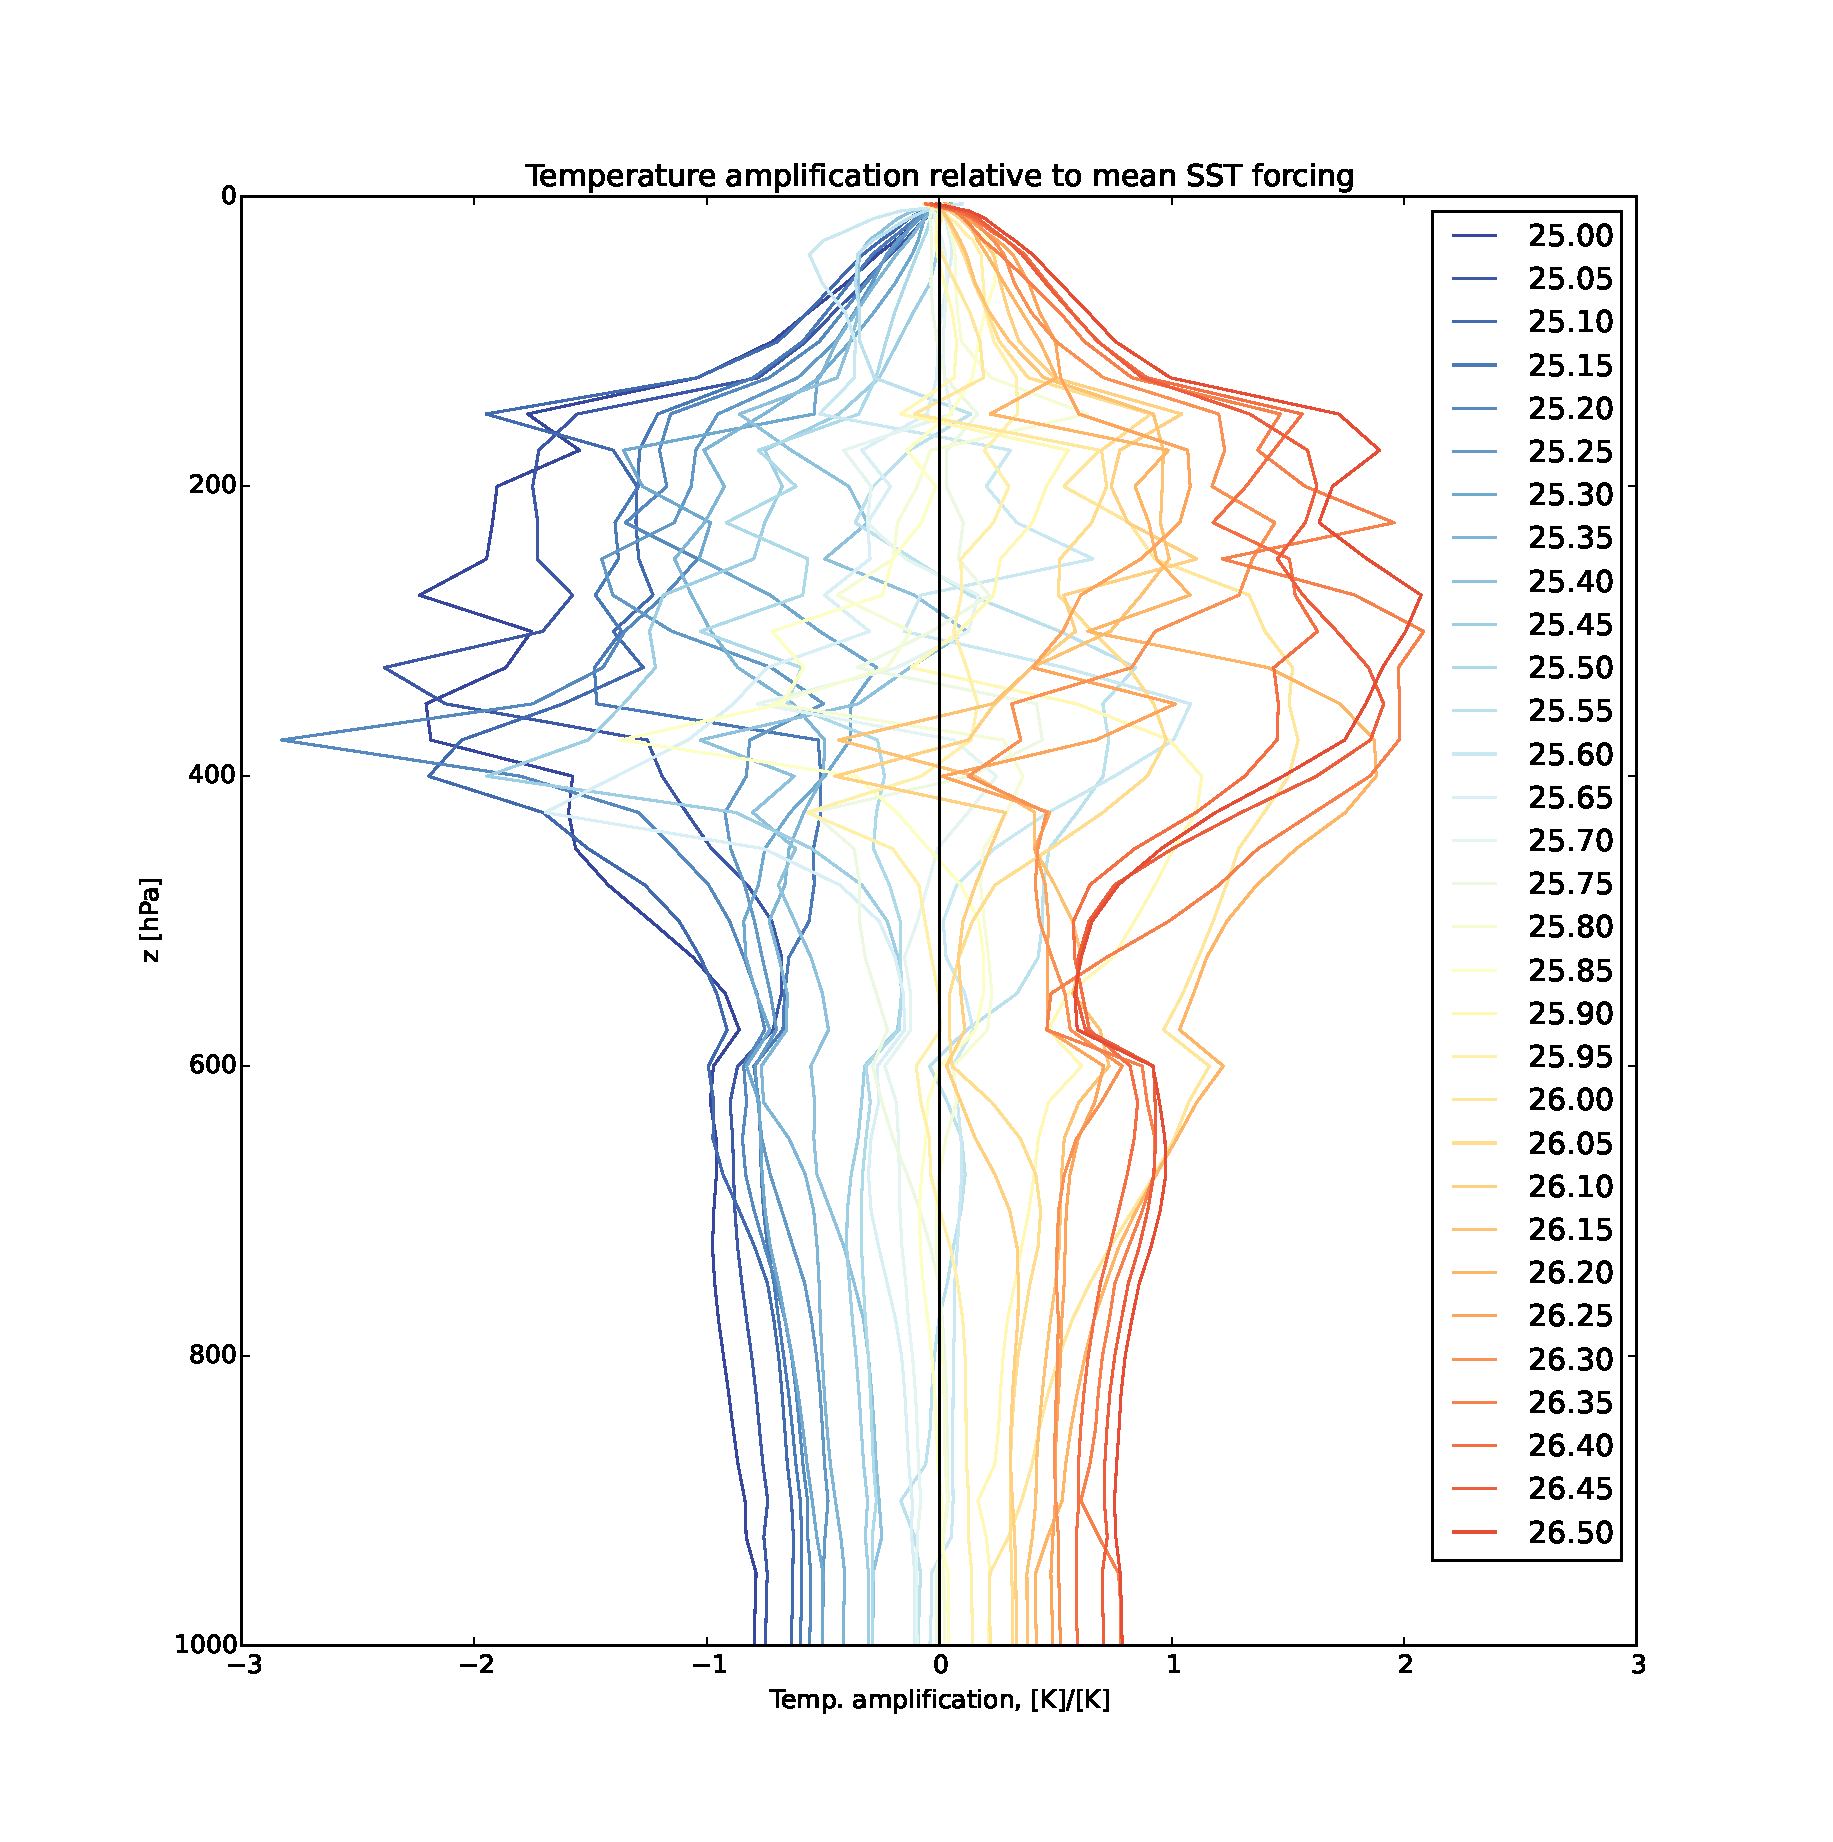
\includegraphics[width=0.5\textwidth]{sstinc_prof_temp_mean.eps}
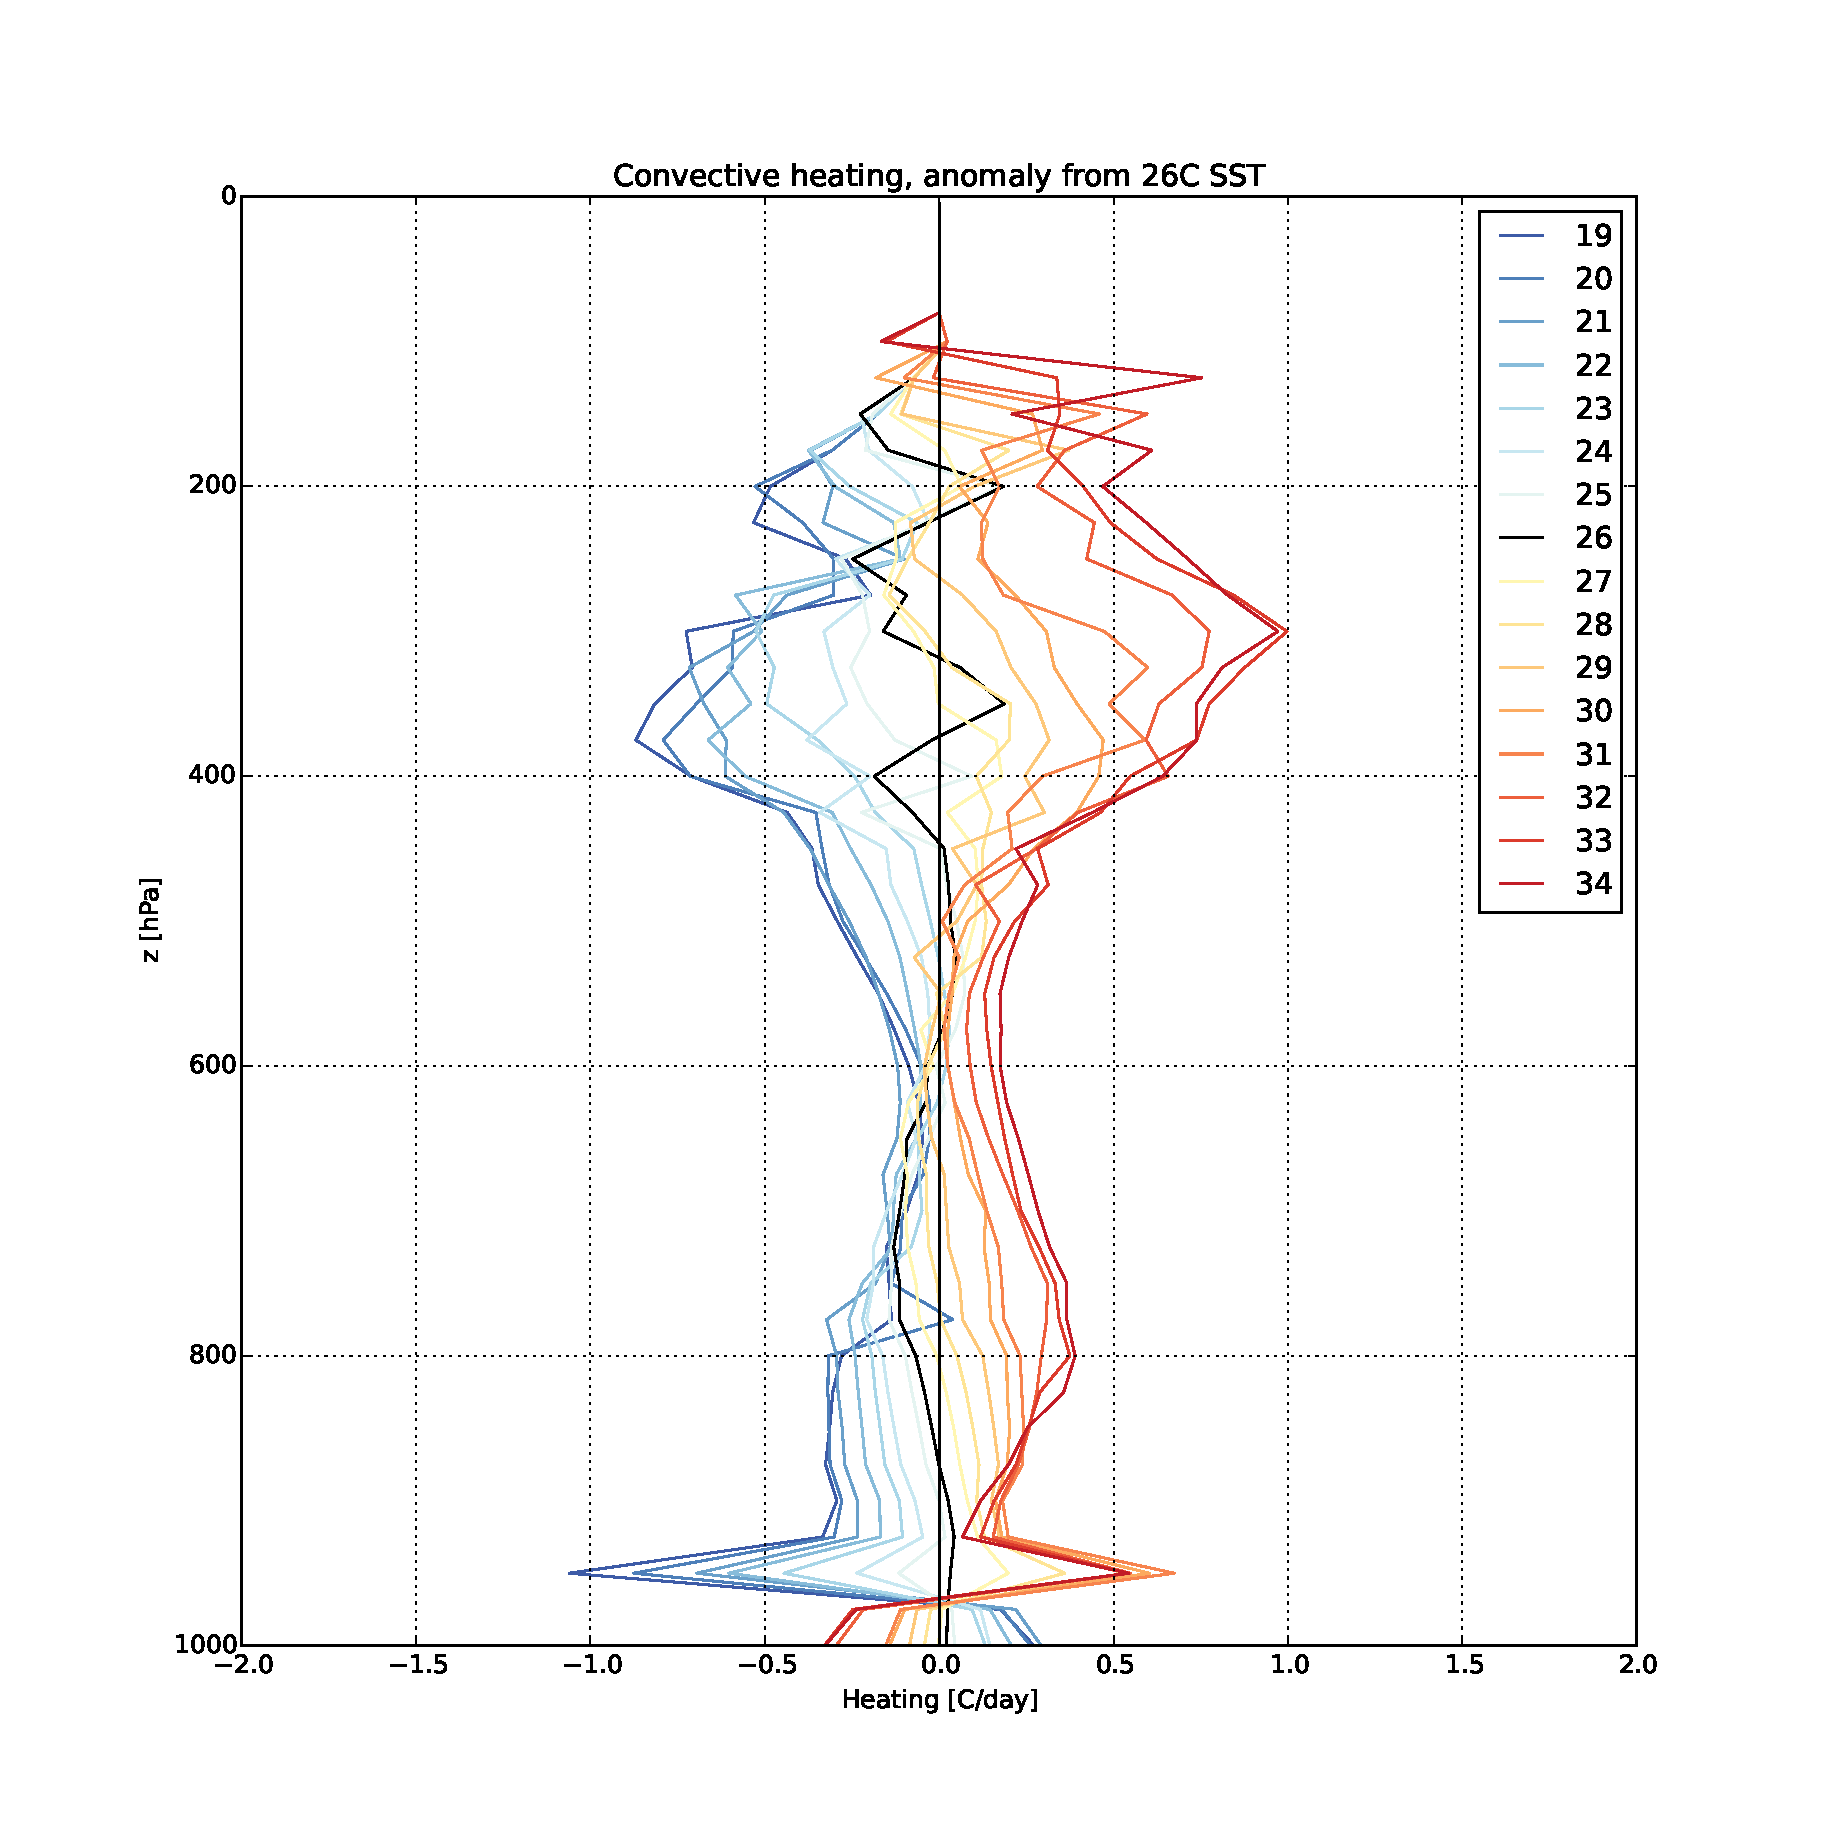
\includegraphics[width=0.5\textwidth]{enso_prof_cq_meananom.eps}
\caption{Heating and temperature profiles for the SCM. a) Temperature anomaly 
	relative to mean profile for SSTs from \SI{19}{\degreeCelsius} to 
	\SI{34}{\degreeCelsius} b) Amplification relative to the mean profile d) 
	Temperature anomalies relative to mean profile c) Moist convective heating 
rates, anomaly from the mean profile.}
\label{fig:scmsstprof}
\end{figure}

\subsubsection{Values of l/s contrast for varying land/tropos parameters}

Parameter testing was discussed in Chapter \ref{methods} in relation to the 
stability of the model. Here we will discuss parameters affecting physical 
processes, with some results shown in Table \ref{tab:scmrlo}. The simplicity of 
the model means the properties of the land surface are primarily controlled by 
the evaporative fraction. By considering the evaporative fraction as a measure 
of soil moisture the results can be related back to observations and GCMs 
results.  The evaporative fraction was found to be the strongest controlling 
factor of the value of $R_{l/o}$, in all scenarios a decrease in evaporative 
fraction lead to an increas in $R_{l/o}$. When using the model in WTG mode it is 
possible to adjust the pressure at which the temperature profile remains fixed 
(PFixT).  It would seem likely that this would influence the value of $R_{l/o}$; 
as the pressure at which the profile remains fixed increases there is more 
potential for the temperature below this to vary.  However it was found that 
PFixT had no clear influence on $R_{l/o}$, implying the variation in temperature 
below the level of the fixed temperature profile is not being significantly 
impacted by the specifics of the model setup. This is a positive outcome, as a 
dependance of $R_{l/o}$ on PFixT would indicate a dependance on a non-physical 
model parameter. Instead we see that we can simulate control of the tropical 
troposphere by tropical oceans and get robust values of $R_{l/o}$.

Overall the values of $R_{l/o}$ are within a realistic range, from 1.1 to 1.6.
Even for the very moist surface -- an evaporative fraction on 0.7 -- the values 
are similar the tropical values from observations ($R_{l/o, obs} =1.19$), and 
the ENSO-Slab run ($R_{l/o, enso} =1.17$), while the CMIP5 ($R_{l/o,cmip} 
=1.35$) and the AMIP run ($R_{l/o, amip} =1.26$) tropical values are closer to 
corresponding values for an evaporative fraction of 0.5. We can compare the 
comparitave variability and co-variability of the land and ocean columns by 
looking at the ratio of standard deviation and the correlation between the 
columns. It is primarily the ratio of standard deviation which is causing the 
increase in $R_{l/o}$ with decreasing evaporative fraction, as the correlation 
between the land and ocean columns, which is around 0.7, doesn't change 
significantly. Although we can't measure changes in the observation and GCM 
values of the ratio of standard deviation or correlation with changing surface 
moisture, we can see that the tropical values are similar to the single column 
model, with correlation of around 0.8 and ratio of standard deviation of around 
1.4.  The consistency of these statistics between the single column model and 
  observations and GCMs are at least an indication that aspects of the 
  relationship between the land and ocean are well represented by the single 
  column model. The single column model results also indicate a strong 
  dependance of the magnitude of $R_{l/o}$ on surface moisture availability.


\begin{center}
	\begin{table}[ht]
		\caption{Land/Ocean contrast in single column model, using WTG over lad 
		surfaces}
		\label{tab:scmrlo}
		\scriptsize
	\begin{tabular}{ l  c  c  c }
		\textit{Evap Fraction}		& 0.3   & 0.5  & 0.7 \\ \hline
		\textbf{PFixT 800hPa}\\%\hline
		$R_{l/o}$  							& 1.41  & 1.43 & 1.18\\ %\hline
	Corr.							& 0.57  & 0.78 & 0.64\\ %\hline
	Ratio STD           			& 2.48  & 1.84 & 1.60\\ \hline
		\textbf{PFixT 700hPa}\\%\hline
		$R_{l/o}$  							& 1.39  & 1.30 & 1.15\\ %\hline
	Corr.							& 0.50  & 0.77 & 0.76\\ %\hline
	Ratio STD           			& 2.76  & 1.68 & 1.52\\ \hline
		\textbf{PFixT 600hPa}\\%\hline
		$R_{l/o}$  							& 1.63  & 1.25 & 1.11\\ %\hline
	Corr.							& 0.70  & 0.79 & 0.78\\ %\hline
	Ratio STD           			& 2.35  & 1.58 & 1.42\\ \hline
	\end{tabular}
	\end{table}
\end{center}

% \clearpage

\subsubsection{Atmospheric profiles}
We will now look at the atmospheric temperature profiles, focusing on one set of 
runs from the single column model. The run with a PFixT (pressure above which 
the temperature profile remains fixed) of \SI{600}{\hecto\pascal} and 
evaporative fraction of 0.3 was chosen because the low evaporative fraction 
resulted in larger deviations between the temperature profiles of the land and 
ocean columns. The results from other runs were similar but of different 
magnitude. \\
\citet{Byrne2013a} outline a mechanism for the global warming land/ocean 
contrast based on the height of the lifting condensation level, as discussed in 
Chapter \ref{sec:logw}. A schematic of the potential temperature ($\theta$) 
profile is shown in the Figure \ref{fig:bo_fig1}. It demonstrates that due to a 
difference in LCL heights the temperature difference between land and ocean is 
dependent on the saturated moist adiabatic lapse rate ($\Gamma_m^*$), and as 
$\Gamma_m^*$ reduces with warming, the difference between land and ocean 
increases.

\begin{figure}[ht]
\includegraphics[width=0.5\textwidth]{{byrne_ogorman_fig1}.png}\\
\caption{Figure 1 from \citet{Byrne2013a}. A schematic of the potential 
temperature}
\label{fig:bo_fig1}
\end{figure}

Comparing this to the profile of $\theta$ in Figure \ref{fig:scmthprof} a) we 
see some similarity in the mean profile (the black line), due the different LCL 
heights, but it is clear that the land profile diverges from the ocean column 
$\Gamma_m^*$ above the LCL. There is also no significant change in the ocean 
column $\Gamma_m^*$ in between the land and ocean LCL levels, which differs form 
the Byrne \& O'Gorman theory. The changes are more easily seen in Figure 
\ref{fig:scmthprof} c) and d). For this figure the SST values were grouped into 
five mean values with the intention of showing the evolution of the change away 
from the mean value (?). If $\Gamma_m^*$ between the land and ocean LCLs were 
controlling the land/sea contrast then the warmest and coolest anomalous ocean 
column (dashed) profiles in \ref{fig:scmthprof} d) would be seen to flatten from 
\SI{950}{\hecto\pascal} to \SI{900}{\hecto\pascal}, instead they are mostly 
vertical. The land (solid) profiles show where the amplification is occuring.  
The largest change in the warmest and coolest profile is occuring around 
\SI{950}{\hecto\pascal} to \SI{900}{\hecto\pascal}. This is due to an increase 
(decrease) in the height of the LCL with warming (cooling). The contrasting 
$\Gamma_m^*$ and dry adiabatic lapse rate ($\Gamma_d$) gradients means that a 
small change in the LCL over land leads to large change in the surface 
temperature. The warmest and coolest land profiles also show a significant 
deviation from the mean above the LCL, around \SI{900}{\hecto\pascal} to 
\SI{800}{\hecto\pascal}.  


\begin{figure}[ht]
\includegraphics[width=0.5\textwidth]{{land_thetaprof_e3_p600}.eps}
\includegraphics[width=0.5\textwidth]{{land_deltatheta_e3_p600}.eps}\\
\includegraphics[width=0.5\textwidth]{{land_thetaprof_fifth_e3_p600}.eps}
\includegraphics[width=0.5\textwidth]{{land_deltatheta_fifth_e3_p600}.eps}
\caption{Profiles of theta (a), change in theta from mean theta value (b), 
change in theta from mean, all profiles averaged into five bins (c and d). Shows 
that extreme values (both positive and negative) change the most.}
\label{fig:scmthprof}
\end{figure}

\clearpage

\subsubsection{Surface Temperature Relationships}
To understand the factors controlling the land surface temperature $T_{land}$ of 
the single column model we will look at relationships between $T_{land}$ and a 
number of variables, beginning with $T_{land}$ verse the SST used to generate 
the imposed temperature profile, shown in Figure \ref{fig:scm_tlandsst}. The 
regression lines represent $R_{l/o}$ and show the increase of $R_{l/o}$ with 
decreasing evaporative fraction. A large amount of variability is also evident 
in the response of $T_{land}$ to the imposed temperature profile, this is a due 
to the interaction between clouds and radiation and is discussed further in 
Chapter \ref{instability}.  Despite the variability, model runs with different 
values of PFixT, domain size, vertical resolution and other parameters show 
similar relationships between $T_{land}$, SST and evaporative fraction.

\begin{figure}[ht]
\includegraphics[width=0.6\textwidth]{{land_anom_intvar_tsurf_p600}.eps}
\caption{Relationship between $T_{land}$ and SSTs}
\label{fig:scm_tlandsst}
\end{figure}

Looking now at how the SST generated temperature profiles influence the 
variables in the land column, and how those variables corelate with $T_{land}$; 
Figure \ref{fig:scm_SSTVar} shows the anomalous SST plotted against the 
anomalous values of relative humidity, longwave and shortwave radiation and 
precipitation.  The SST is that used to generate the imposed temperature profile 
and the variables are from the land column. There are few significant 
relationships between the forcing SSTs and the land column variables. Table 
\ref{tab:scm_SSTVar} shows that the relative humidity is partially related to 
the SST forcing, although the highest correlation is still only -0.41, and no 
other correlations are above 0.30. In contrast there are clear relationships 
between the relative humidity, longwave and shortwave radiation and cloud 
fraction and $T_{land}$. So we see that while the imposed temperature profiles 
have a high correlation with the resultant surface temperatures in the mean 
values, as shown in Table \ref{tab:scm_rlo}, variability in the convection 
scheme has a large influence on surface temperatures leading to the variability 
shown in Figure \ref{fig:scm_tlandsst}.

\begin{center}
	\begin{table}[ht]
		\caption{Correlation between forcing SST values variables governing the 
		land column surface response.}
		\label{tab:scm_SSTVar}
		\scriptsize
	\begin{tabular}{ l  c  c  c }
		\textit{Evap Fraction:}		& 0.3   & 0.5  & 0.7 \\ \hline
		\textbf{Relative Humidity}\\%\hline
	Corr.							& -0.41  & -0.33 & -0.26\\ %\hline
		\textbf{Shortwave Radiation}\\%\hline
	Corr.							& 0.17  & 0.28 & 0.28\\ %\hline
		\textbf{Longwave Radiation}\\%\hline
	Corr.							& 0.15  & 0.24 & 0.27\\ %\hline
		\textbf{Cloud Fraction}\\%\hline
	Corr.							& -0.14  & -0.00 & -0.06\\ %\hline
	\end{tabular}
	\end{table}
\end{center}

\begin{figure}[ht]
\includegraphics[width=0.5\textwidth]{{land_anom_intvar_rh_p600}.eps}
\includegraphics[width=0.5\textwidth]{{land_anom_intvar_lw_p600}.eps}
\includegraphics[width=0.5\textwidth]{{land_anom_intvar_sw_p600}.eps}
\includegraphics[width=0.5\textwidth]{{land_anom_intvar_clf_p600}.eps}
\caption{Relationship between; relative humidity, longwave radiation, shortwave 
radiation and cloud fraction, and land and ocean surface temperature}
\label{fig:scm_SSTVar}
\end{figure}

\clearpage


\subsubsection{Variability and instability - Role of convection}
\label{instability}
Given the large variability in $T_{tropos}$ and the weak connection between the 
imposed temperature profile and convection, a discussion of the stability of the 
model is in order. The timeseries in Figure \ref{fig:scmts} a)-c) demonstrate a 
range of chaotic behaviours. For many runs being forced with a cooler 
temperature profile we see regular oscillations, it should be noted their is no 
diurnal cycle in the model. For forcing with higher temperatures we see a 
decoupling of the surface temperatures and the imposed temperature profile which 
results in a lower surface temperature from a higher forcing temperature. The 
oscillations and the instability are due to the interaction of clouds and 
radiation. This is easily demonstrated as interaction between the convection and 
radiation schemes in the model can be turned off. The resultant timeseries, 
shown in Figure \ref{fig:scmts}, quickly reaches a stable equilibrium 
temperature. 

\begin{figure}[ht]
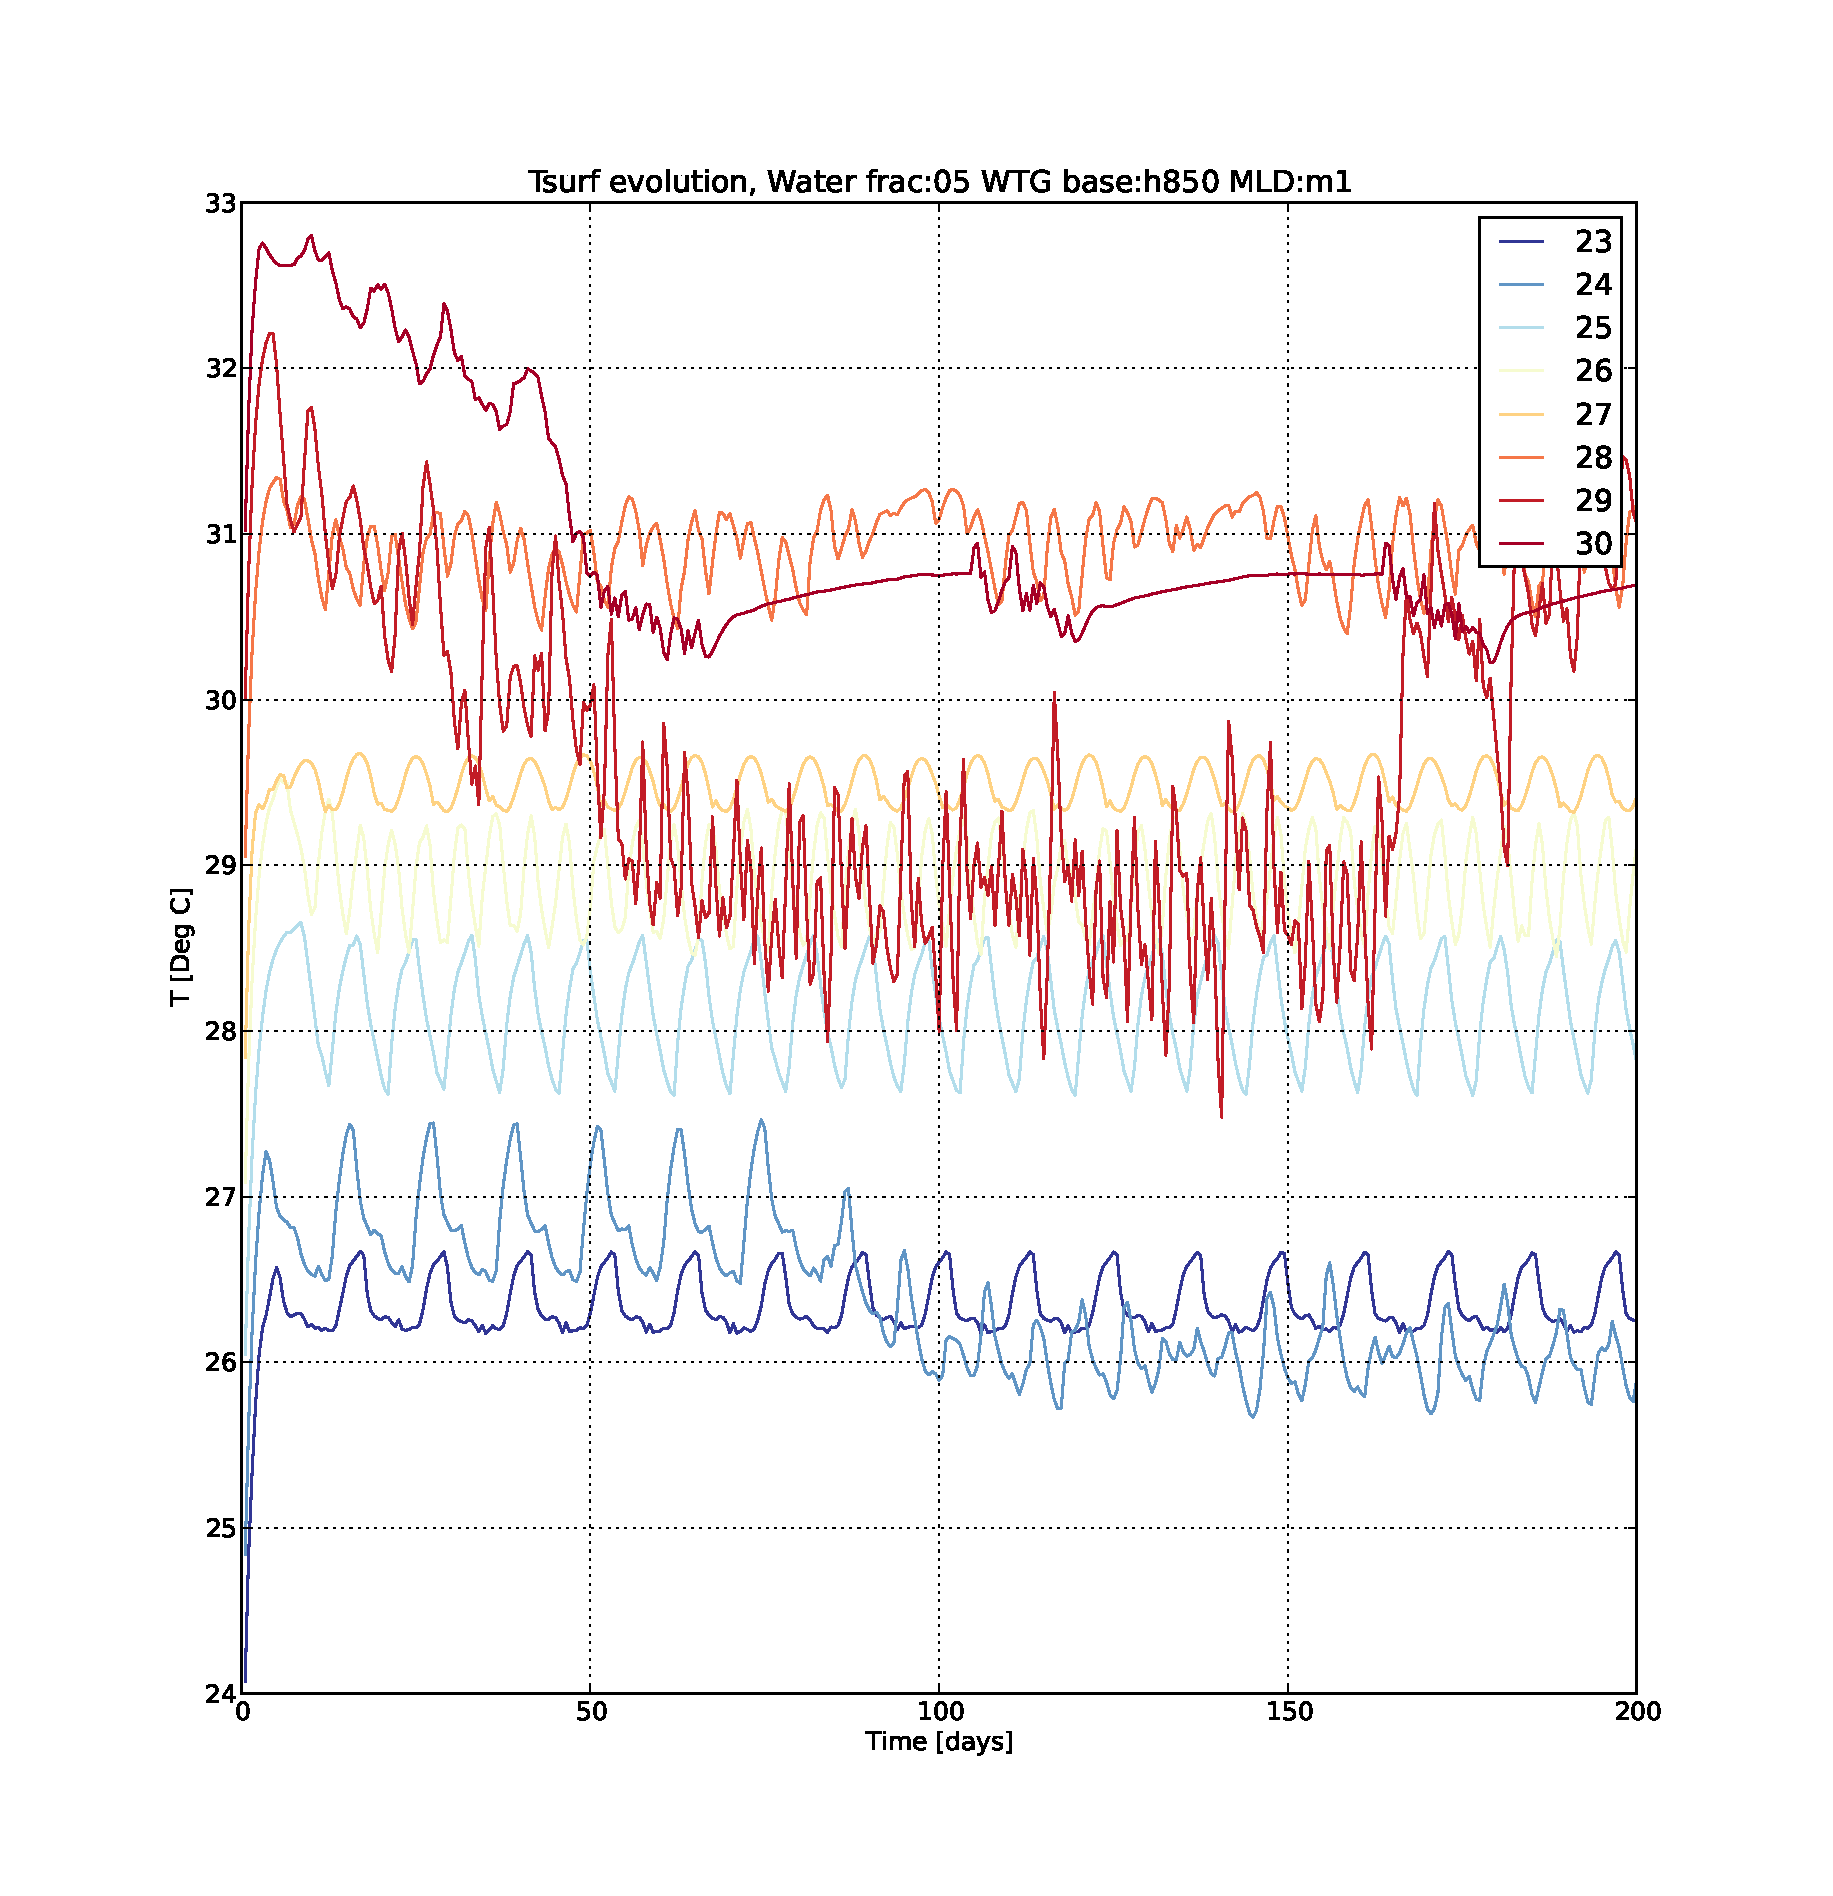
\includegraphics[width=0.4\textwidth]{land_Tsurf_05_m1_h850.eps}
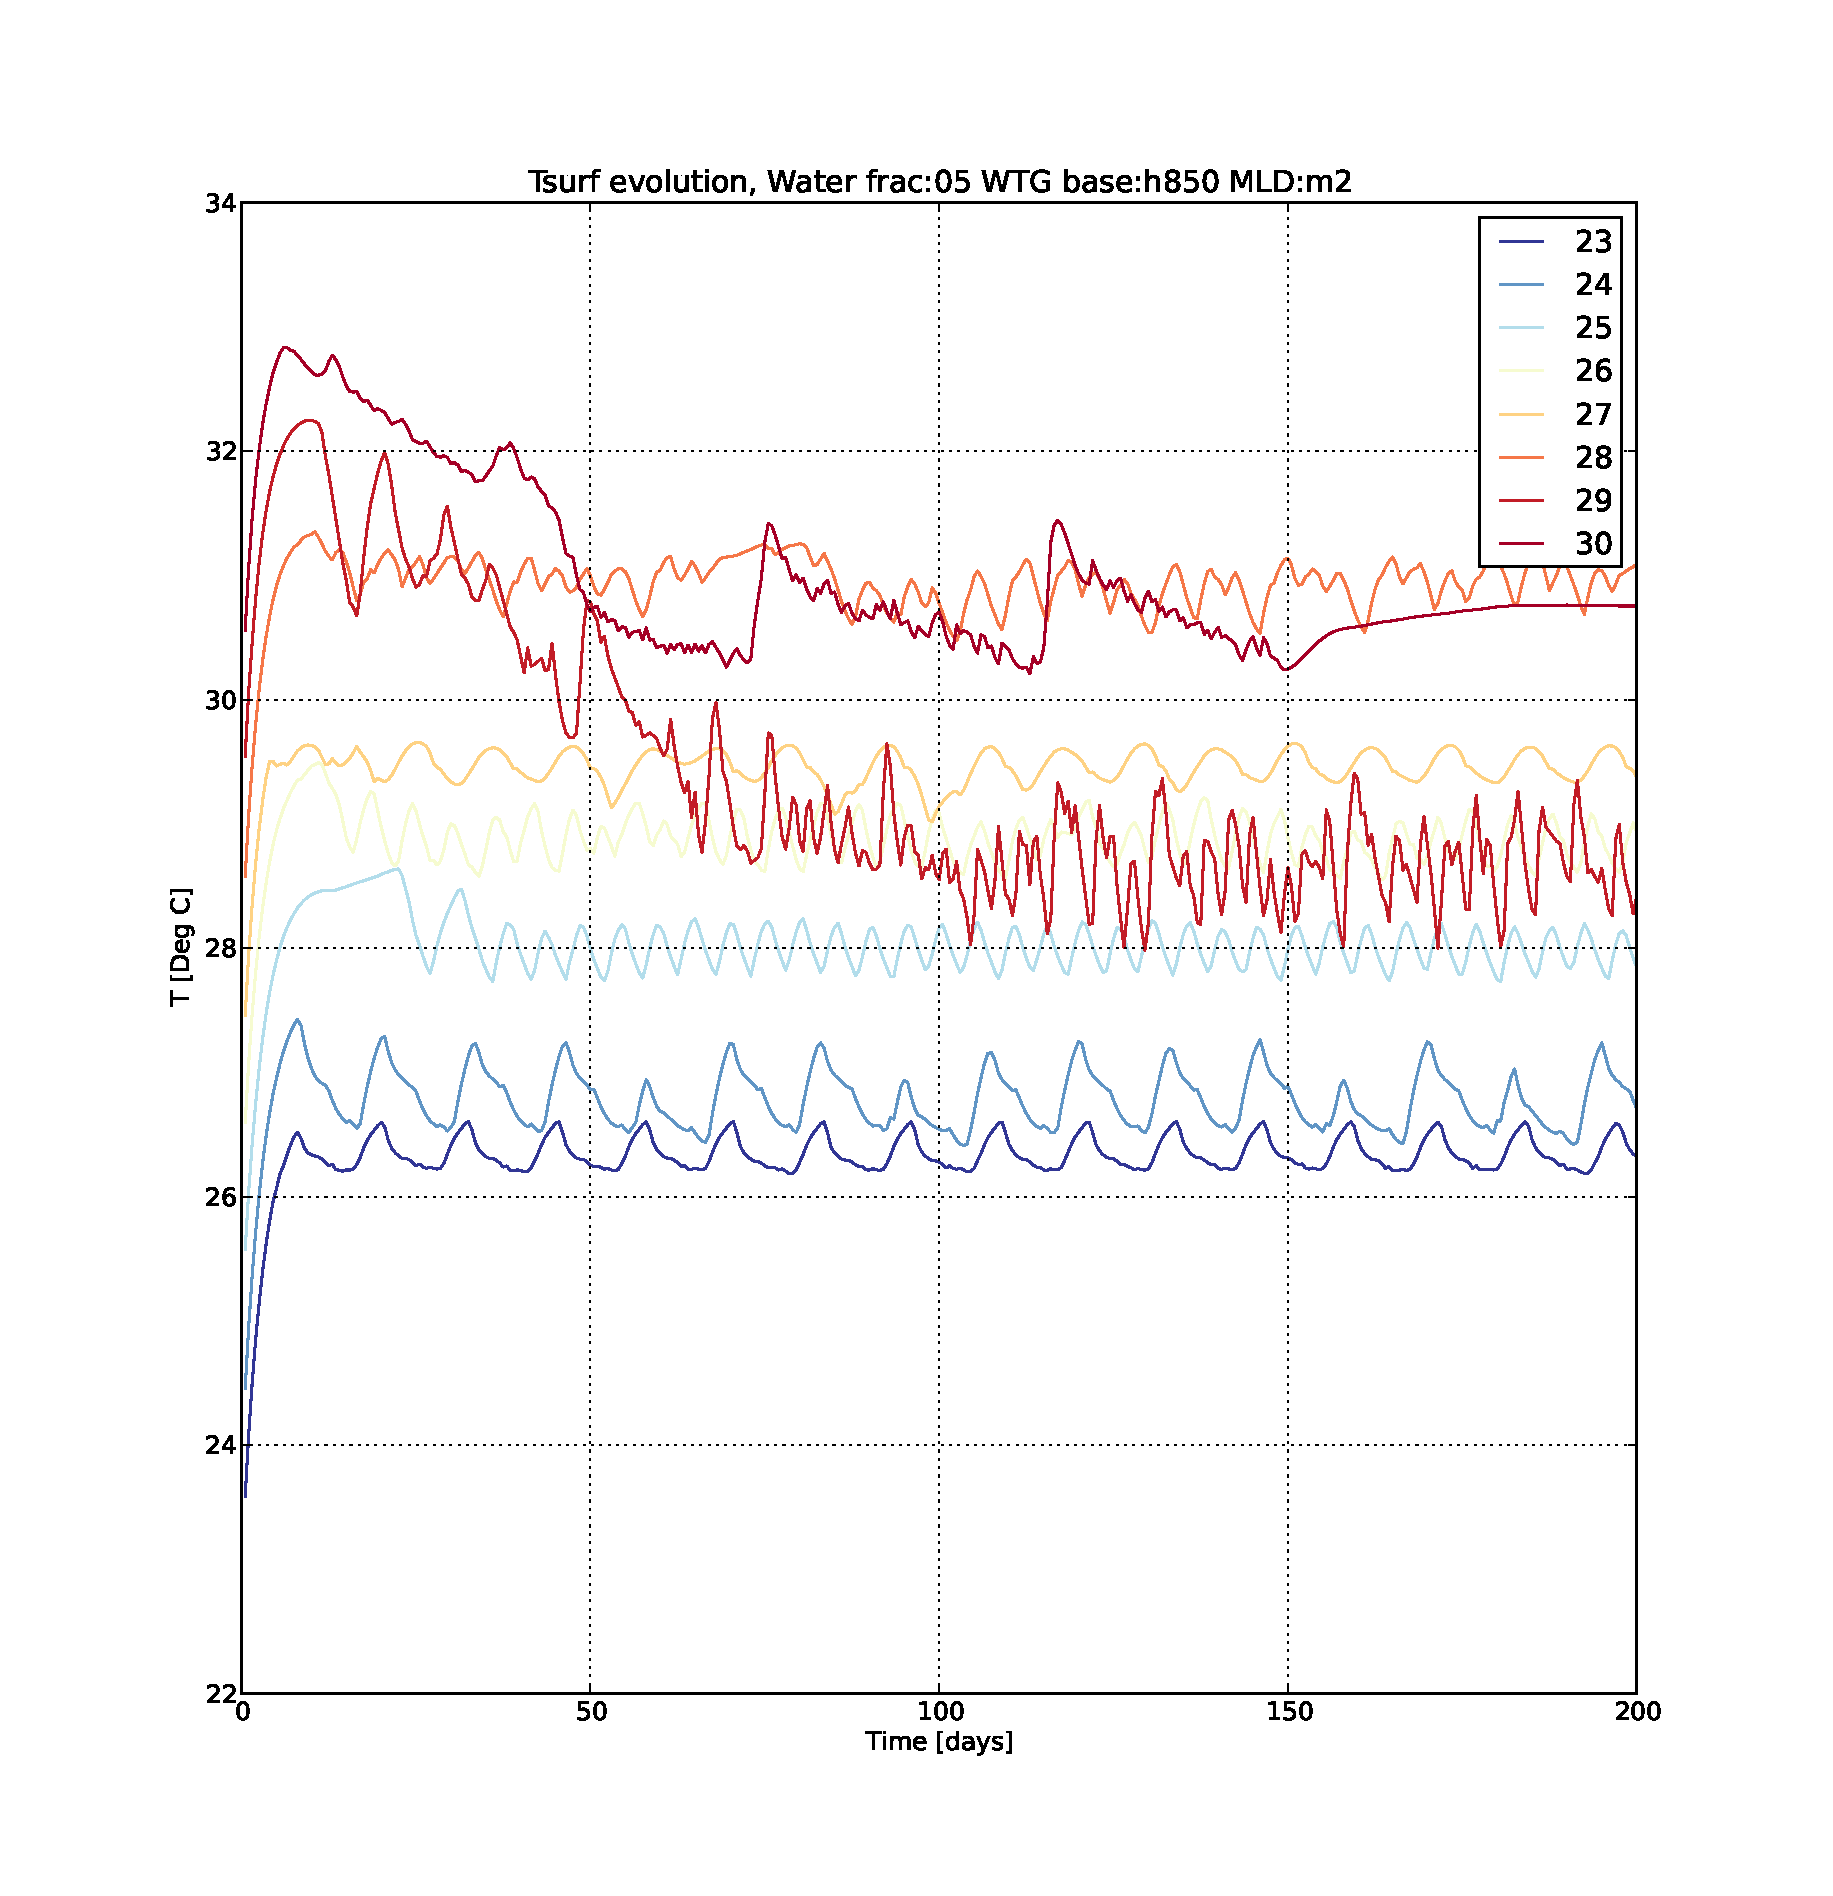
\includegraphics[width=0.4\textwidth]{land_Tsurf_05_m2_h850.eps}\\
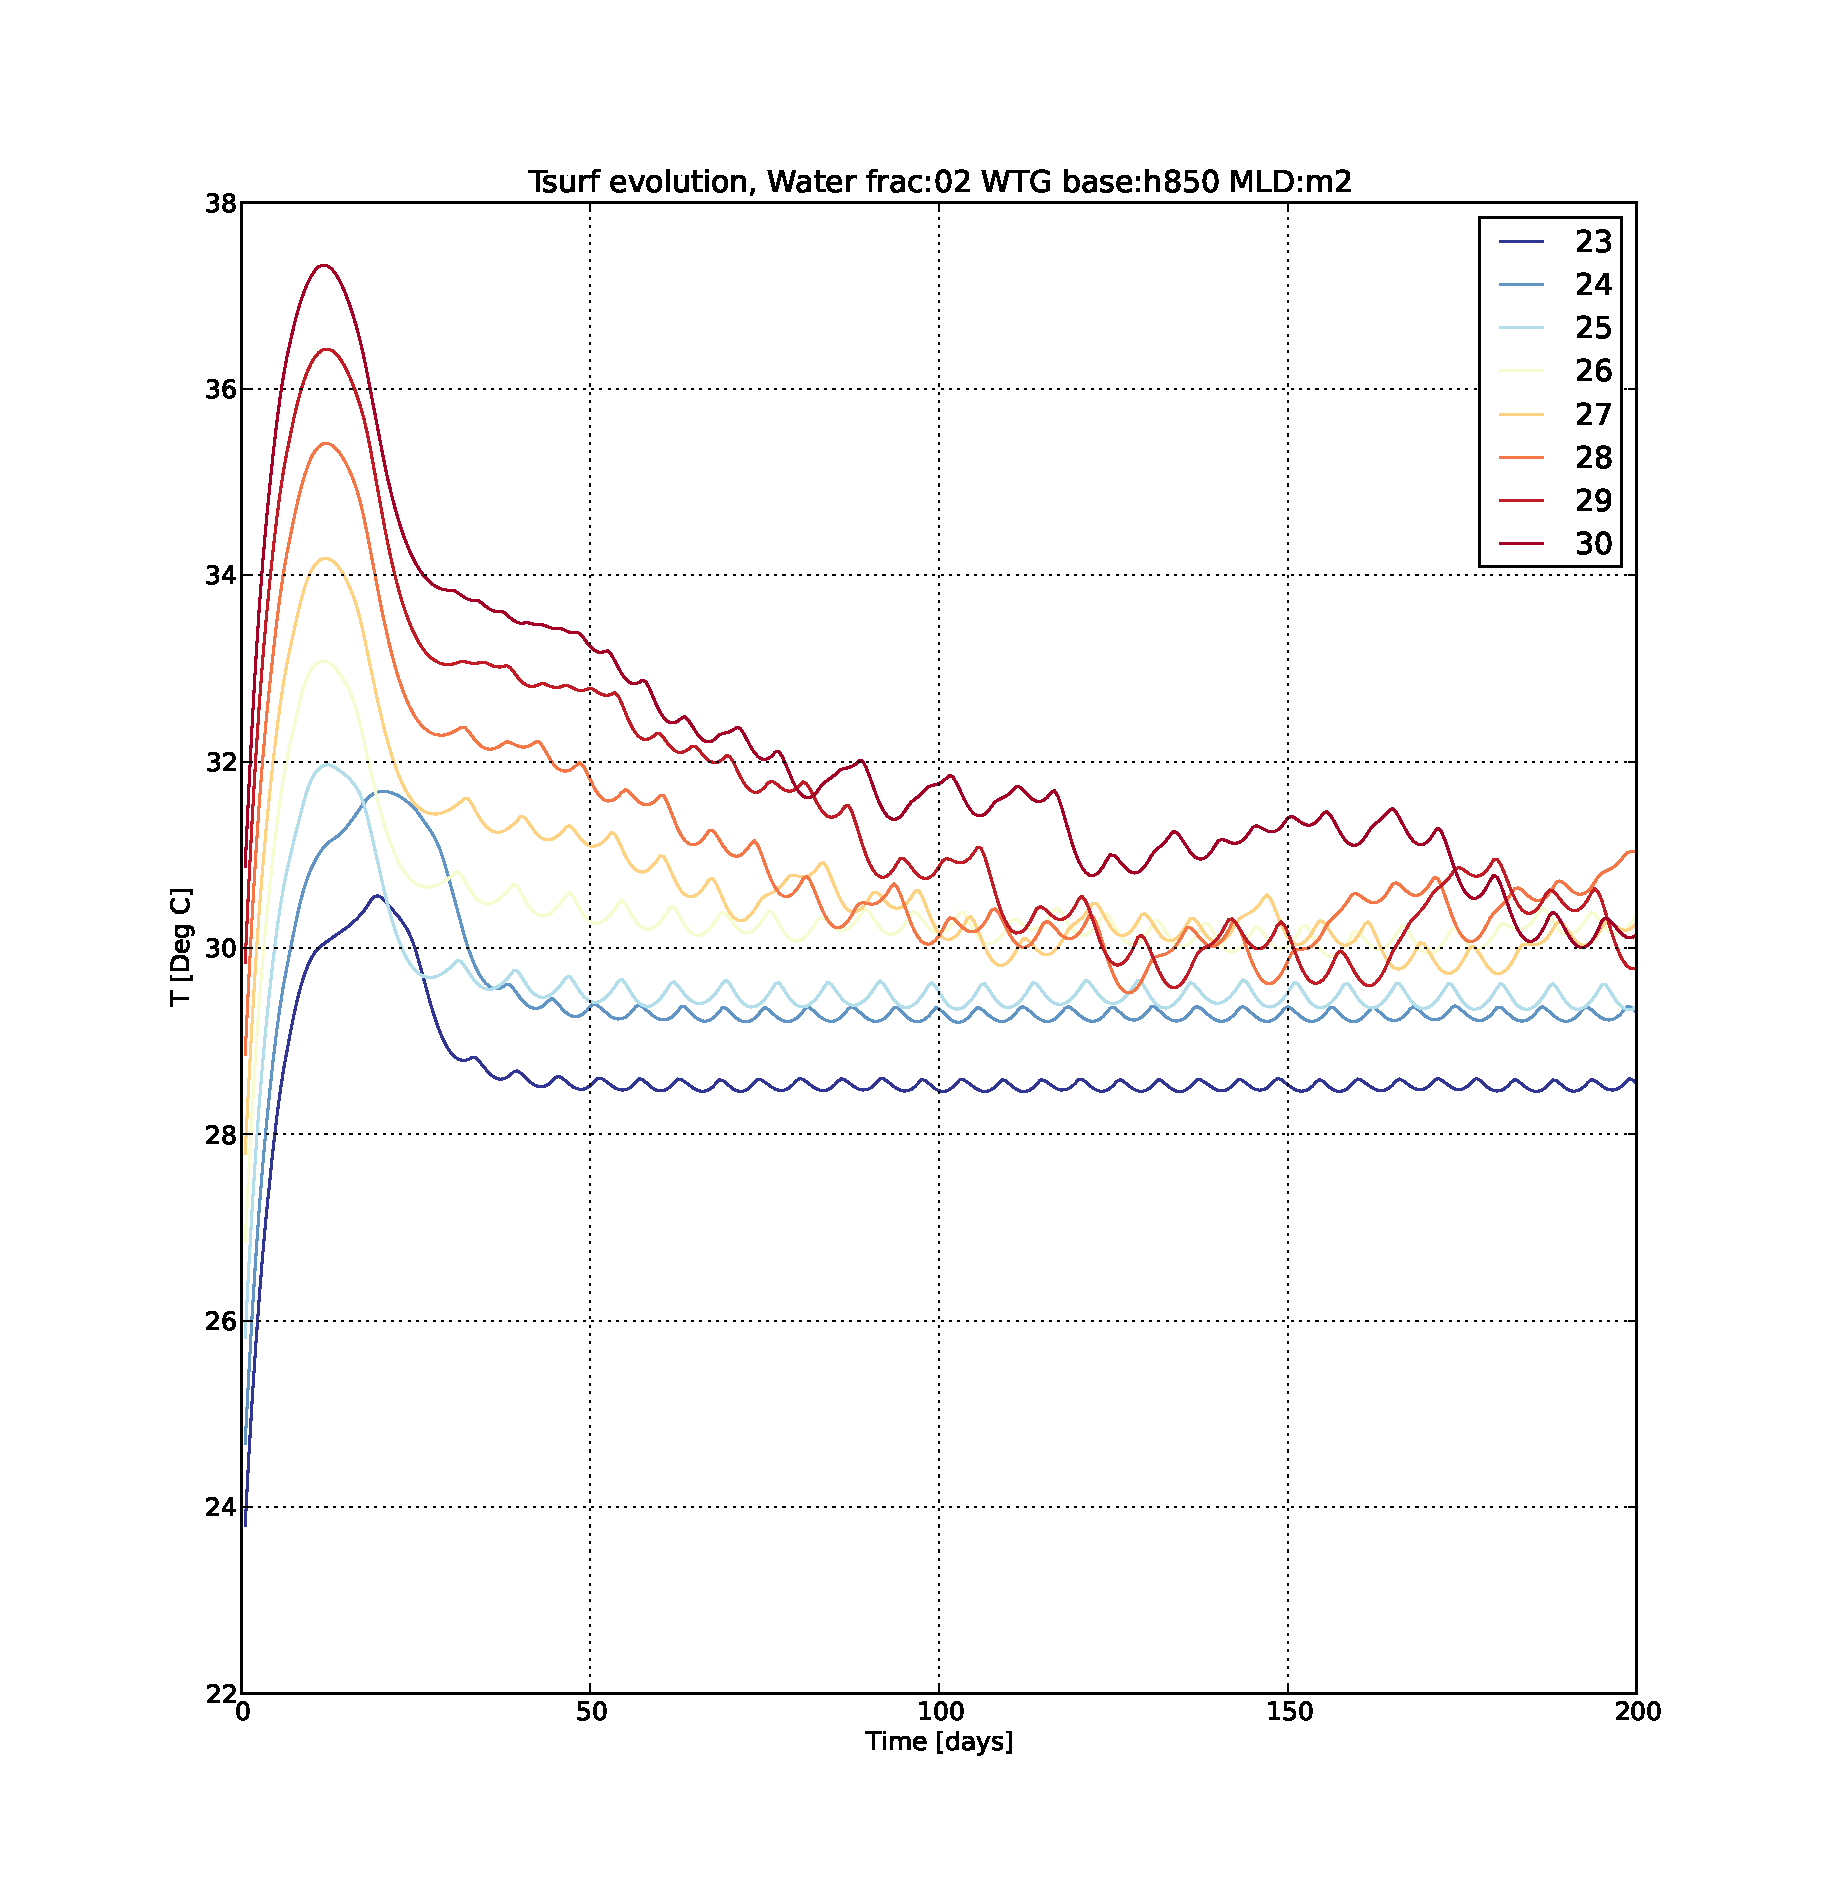
\includegraphics[width=0.4\textwidth]{land_Tsurf_02_m2_h850.eps}
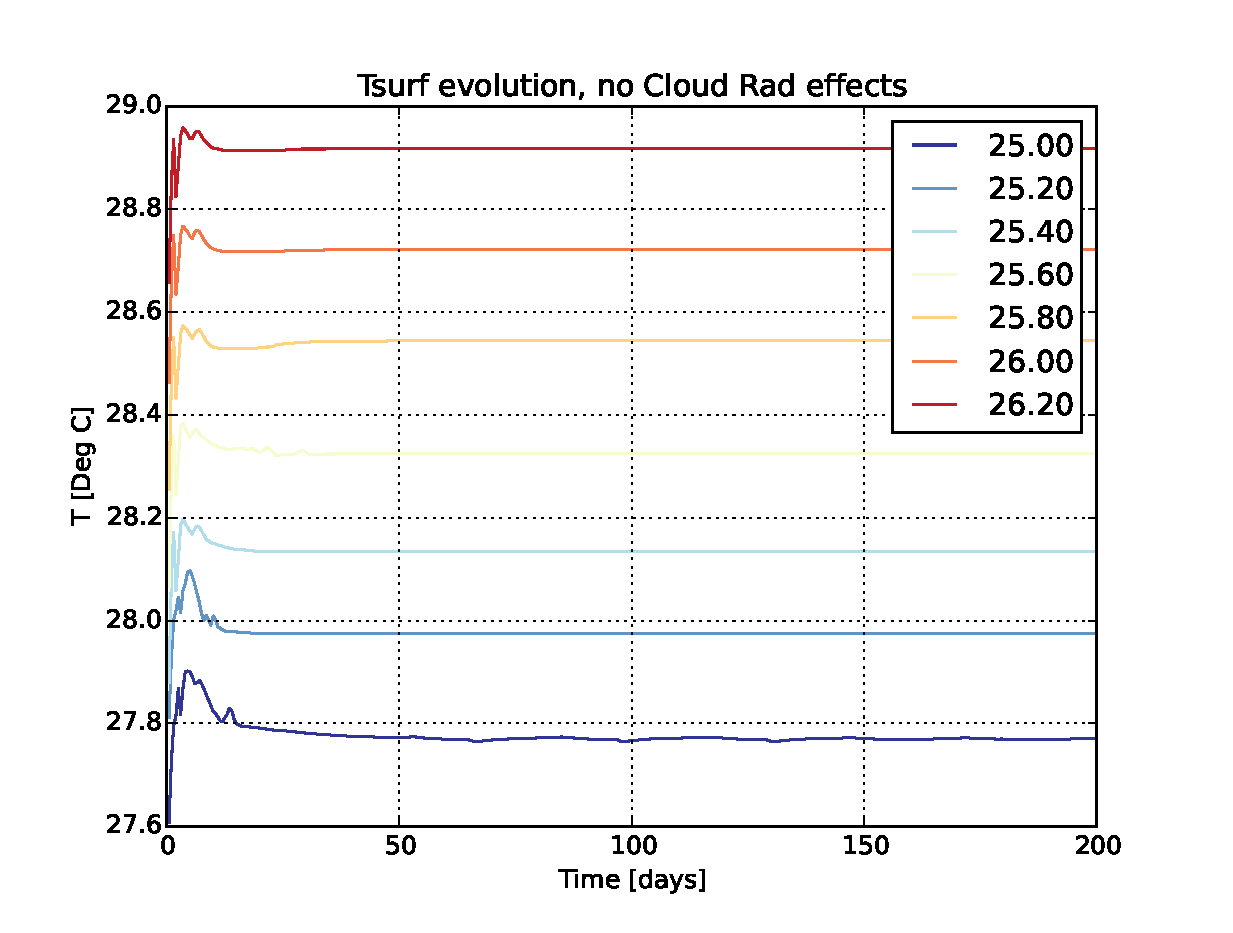
\includegraphics[width=0.4\textwidth]{land_nir_Tsurf.eps}\\
\caption{Timeseries of Tsurf in SCM forced with tropospheric temperature 
profile.}
\label{fig:scmts}
\end{figure}



\clearpage

\subsection{Experiments with a Two-Dimensional Model}

The single column model in weak temperature gradient mode offered a promising 
and novel approach to investigating the land/sea contrast and the role of ocean 
forcing.  However, a few issues remained; the instability of the model under 
certain conditions has the potential to lead to unrealistic results, and 
disabling the interaction between the convection and radiation schemes damped  
any land response. In addition, the assumptions of the WTG approximation are 
only valid in the tropics, a limiting factor when attempting to explain the 
regional differences in the land response. In order to continue using the column 
model while avoiding these issues a multi column setup was used.\\
The full description of the setup is outlined in Chapter \ref{methods}. To 
reiterate, the model can be run with one or more ocean and one or more land 
columns. A number of different geometries of land and ocean columns were tested, 
with the resultant $R_{l/o}$ values shown in Table \ref{tab:tdm_Rlo}. Due to the 
instability of the model, the interaction between clouds and radiation was 
turned off for these runs. When the cloud/radiation interaction was switched off 
in the single column model in WTG mode it lead to a strong damping of $R_{l/o}$.  
In contrast, in the multi column model the imposed SSTs are still able to 
strongly influence the land surface. The values of $R_{l/o}$  are lower than the 
single column model and an amplification of the imposed SSTs is only seen for 
evaporative fractions below 0.3, and once again they increase with decreasing 
evaporative fraction.   

\begin{center}
	\begin{table}[ht]
		\caption{Land/Ocean contrast in two dimensional model}
		\label{tab:tdm_Rlo}
		\scriptsize
	\begin{tabular}{ l  c  c  c  c  c }
		\hline
		\textit{Evap Fraction}	& 0.05  & 0.10 & 0.30  & 0.50  & 0.70 \\ \hline
		\textbf{1 Ocean, 1 Land}\\
		$R_{l/o}$ 					& 1.28  & 1.23 & 1.03  & 1.05 & 1.00\\ 
		Corr.					& 0.98  & 1.00 & 1.00  & 1.00 & 1.00\\ %\hline
		Ratio STD          		& 1.30  & 1.23 & 1.03  & 1.05 & 1.00\\ \hline
		\textbf{3 Ocean, 1 Land}\\
		$R_{l/o}$ 					& 1.17  & 1.12 & 1.03  & 1.01 & 0.98\\ %\hline
		Corr.					& 1.00  & 1.00 & 1.00  & 1.00 & 1.00\\ %\hline
		Ratio STD          		& 1.17  & 1.12 & 1.03  & 1.01 & 0.98\\ \hline
		\textbf{1 Ocean, 3 Land}\\
		$R_{l/o}$ 					& 1.13  & 1.10 & 1.02  & 0.94 & 0.86\\ %\hline
		Corr.					& 1.00  & 1.00 & 1.00  & 1.00 & 1.00\\ %\hline
		Ratio STD          		& 1.13  & 1.10 & 1.02  & 0.94 & 0.86\\ \hline
		\textbf{3 Ocean, 3 Land}\\
		$R_{l/o}$ 					& 1.16  & 1.11 & 1.00  & 0.96 & 0.91\\ %\hline
		Corr.					& 1.00  & 1.00 & 1.00  & 1.00 & 1.00\\ %\hline
		Ratio STD          		& 1.16  & 1.11 & 1.00  & 0.96 & 0.91\\ \hline
	\end{tabular}
	\end{table}
\end{center}

The single and 2D column model was used with the purpose of understanding the 
vertical structure of the land/ocean temperature contrast. We can see from Table 
\ref{tab:tdm_Rlo} that -- when using small evaporative fractions -- we can 
reproduce the magnitude of $R_{l/o}$ so now we will compare the vertical 
structure with the GCM results. Using the same technique as with the GCM, we use 
the regression coeffecient between the temperature at the surface and each model 
level to plot the response to warming and cooling above ocean and land surfaces.  
Figures \ref{fig:tdm_regprof} a) and b) have some key similarities and 
differences; the ocean profiles are both very similar, they feature the large 
amplification around \SIrange{200}{400}{\hecto\pascal} due to moist convection, 
as well as a local maximum at the freezing level at \SI{600}{\hecto\pascal}.  
Comparing the profiles above land we see a large difference above 
\SI{500}{\hecto\pascal}. In the GCM the moist convective amplification is damped 
above land whereas in the 2D column model the two profiles follow each other 
closely. This doesn't necessarily imply the presence of moist convection in the 
land columns, merely that the land and ocean are more tightly linked in the 2D 
model. Allowing for this descrepency the GCM and column model are very similar.  
In the area above \SI{800}{\hecto\pascal} the land/ocean contrast disappears and 
below \SI{800}{\hecto\pascal} the land and ocean profiles diverge to give 
similar values of $R_{l/o}$. From Figure \ref{fig:tdm_regprof} we can assume 
that there will be difference in the land surface response in the GCM and 2D 
column model due to the descrepency in the upper troposphere response, but 
importantly the lower atmospheric response appears similar, making the 
simplified model suitable for further investigation of the land/ocean 
temperature contrast and the role of ocean forcing.


\begin{figure}[ht]
	\includegraphics[width=0.5\textwidth]{{presub_fsstreg_prof_ocensfc_e0.05}.eps}
	\includegraphics[width=0.5\textwidth]{{linreg_ocean_profile}.eps}
	\caption{Land/sea contrast in TCM}
\label{fig:tdm_regprof}
\end{figure}


\subsubsection{Atmospheric profiles in temp, RH, etc}

The atmospheric profiles of $\theta$ for the single column indicated that a 
changing LCL over land as well as a deviation between land and ocean lapse rates 
above the LCL can lead to $R_{l/o}>1$. We will know look at profiles of $\theta$ 
in the 2D model. The potential iportance of a changing LCL motivated an increase 
in the vertical resolution of the model. The grid was non-uniform with 85 
levels, and a resolution of \SI{5}{\hecto\pascal} between 
\SIrange{980}{800}{\hecto\pascal} and \SI{10}{\hecto\pascal} between 
\SIrange{800}{650}{\hecto\pascal}, with the fine resolution preventing step 
changes in the height of the LCL.  Figure \ref{fig:tdm_prof} doesn't indicate 
any large change in the LCL over land or ocean. Looking more closely at the 
gradient of $\theta$, in Figure \ref{tdm_dthdp}, there is an indication that in 
the ocean column the gradient of $\theta$ above the LCL does become more 
negative with increasing SST, which is the expected result according to the 
Byrne and O'Gorman theory. However, we do see an unusual feature; from 
\SIrange{900}{800}{\hecto\pascal} the land profile is above, or cooler than, the 
ocean profile. This region of warmer ocean/cooler land could have the effect of 
dampening the value of $R_{l/o}$ and is not an expected feature. To understand 
what is happening we will look at the profiles of relative humidity

\begin{figure}[ht]
	\includegraphics[width=0.5\textwidth]{{l3o1_prof_theta_ef0.05_close}.eps}
	\includegraphics[width=0.5\textwidth]{{l3o1_prof_theta_ef0.05}.eps}
	\caption{Atmospheric profiles in the 2D model}
\label{fig:tdm_prof}
\end{figure}

\begin{figure}[ht]
	\includegraphics[width=0.5\textwidth]{{l3o1_prof_dthetadp_ef0.05_close}.eps}
	\caption{Profiles of $D\theta/Dp$ in the 2D model}
\label{fig:tdm_dthdp}
\end{figure}

Regarding the warmer ocean/cooler land, the profiles of relative humidity are 
quite telling. The relative humidity profile in Figure \ref{fig:tdm_rhprof} a) 
is from the same run as Figure \ref{fig:tdm_prof}, it has one ocean and three 
land columns, although just two SSTs are plotted as the results are similar for 
a range of SSTs.  From the surface we see the much higher relative humidity over 
the ocean column then a sudden drop at around \SI{970}{\hecto\pascal}, to the 
extent that the ocean column becomes drier than the land columns. The dry 
region, from \SIrange{940}{800}{\hecto\pascal} coincides with the steeper 
$\theta$ lapse rate. To test whether the model setup with only one ocean column 
is responsible for the dry region, we look at a run with three ocean and three 
land columns. Figures \ref{fig:tdm_rhprof} b) c) and d) all show a similar 
drying in the ocean column. It also shows that the amount of drying is largely 
insensitive to the humidity and moisture of the land columns. The evaporative 
fraction has a large influence on the relative humidity of the ocean columns, 
for example comparing Figure \ref{fig:tdm_rhprof} b), c) and d) which have 
evaporative fractions of 0.05, 0.10 and 0.20 respectively, the near surface 
humidity changes from 45\% to 60\%, however the response of the ocean columns is 
very similar. The difference in the dry region is at most 5\%.

\begin{figure}[ht]
	\includegraphics[width=0.5\textwidth]{{l3o1_prof_rh_ef0.05_close}.eps}
	\includegraphics[width=0.5\textwidth]{{l3o3_prof_rh_ef0.05_close}.eps}
	\includegraphics[width=0.5\textwidth]{{l3o3_prof_rh_ef0.10_close}.eps}
	\includegraphics[width=0.5\textwidth]{{l3o3_prof_rh_ef0.20_close}.eps}
	\caption{Atmospheric profiles of relative humidity}
\label{fig:tdm_rhprof}
\end{figure}

\subsubsection{Circulation response}
To see what is causing the drying in the ocean columns we look at the vertical 
velocity, $\omega$ and circulation using the streamfunction $\psi$ of vertical 
and zonal velocities.  For these variables we use the mean across a range of 
SSTs, as there weren't any significant changes in circulation for varying SSTs.  
The profiles of $\omega$ clearly shows the convection in the ocean columns 
(positive values of $\omega$, which is balanced with sinking motion in the land 
columns. The $\psi$ profile better demonstrates the flow in the model, and shows 
a low level circulation response. Positive values of $\psi$ indicate clockwise 
flow centered at \SI{850}{\hecto\pascal} in the ocean column nearest the land.  
This circulation is responsible for transporting dry air from the land columns.

\begin{figure}[ht]
	\includegraphics[width=0.5\textwidth]{{l3o3_omegal_ef0.05_meansst}.eps}
	\includegraphics[width=0.5\textwidth]{{l85co2_psi_ef0.05_meansst}.eps}
	\caption{Circulation response, Omega, Psi}
	\label{fig:tdm_circ}
\end{figure}

This circulation appears to be significantly influencing the atmospheric 
structure in the ocean column, but is it affecting the ocean's influence of the 
land column, and thus the value of $R_{l/o}$? This drying of the atmosphere 
above the ocean is not present in a large scale across the globe and therefore 
ould be of concern when determining the suitability of this simplifed model.  
Figure \ref{fig:tdm_psi} shows how the low level circulation scales with 
evaporative fraction, such that the drier the land the stronger the low level 
circulation.  Refering back to Table \ref{tab:tdm_Rlo}, $R_{l/o}$ increases with 
decreasing evaporative fraction. If the value of $R_{l/o}$ is related to the 
difference in lapse rates above land and ocean, which in turn is related to the 
difference in humidity, then a drying of the ocean column may lead to a smaller 
difference between the ocean and land columns.\\
Instead, we see that the reduction in humidity is largely insensitive to the 
evaporative fraction (Figure \ref{fig:tdm_rhprof}) and while the strength of the 
low level circulation driving the reduced humidity increases with evaporative 
fraction, the value of $R_{l/o}$ still increases, implying that the drying of 
the ocean column is not significantly affecting the value of $R_{l/o}$, or more 
importantly, the ability of the simplified model to simulate the land/sea 
contrast.



\begin{figure}[ht]
	\includegraphics[width=0.5\textwidth]{{l85co2_psi_ef0.05_meansst}.eps}
	\includegraphics[width=0.5\textwidth]{{l85co2_psi_ef0.10_meansst}.eps}
	\includegraphics[width=0.5\textwidth]{{l85co2_psi_ef0.20_meansst}.eps}
	\includegraphics[width=0.5\textwidth]{{l85co2_psi_ef0.30_meansst}.eps}
	\caption{Circulation response, Psi}
	\label{fig:tdm_psi}
\end{figure}


\clearpage

\subsubsection{Values of l/s contrast for varying land parameters}
We have seen that while the two-dimensional model has a low level circulation 
that dries the ocean column, it is still able to simulate aspects of the 
land/ocean contrast we see in GCMs (i.e. Figure \ref{fig:tdm_regprof}), and it's 
response to surface properties is expected from the lapse rate of theories of 
\cite{Joshi2007} and \cite{Byrne2013a}. We now extend the range of evaporative 
fractions and vary the latitudes to build a picture of the range of $R_{l/o}$ 
values.\\
The model had 3 ocean and 3 land columns and initially was run in a zonally 
orientated domain. At each latitude an appropriate mean SST value, solar zenith 
angle and coriolis parameter were used.  The model was forced with a range of 
SSTs values which varied around the mean value for each latitude, and $R_{l/o}$ 
was calculated for each parameter.	The results, in Figure \ref{fig:tdm_Rlo} 
show the dependence of $R_{l/o}$ on evaporative fraction, but also a decrease 
with latitude, excepting the increase from \SI{0}{\degree} and \SI{10}{\degree}.  
The same experiments were also performed using a meridionally orientated domain, 
where the prescribed SST columns were nearer to the "equator". The values of 
$R_{l/o}$ for the meridional domain show the same tendencies but at first appear 
lower than the zonal domain, however as each column spans \SI{5}{\degree} of 
latitude, if we compare $R_{l/o}$ values of a specific column and compare it to 
the corresponding latitude of the zonally orientated model we see they are quite 
similar, i.e.  Figure \ref{fig:tdm_Rlo} d). The implication is that the 
reduction in the ability of the ocean columns to control SST, and hence a 
reduced $R_{l/o}$ with increasing latitude is due to a combination of lower 
absolute SST values, and reduced transport across the domain. The latter is 
evident in Figure \ref{fig:tdm_Rlo} c), which shows the mean relative humidity 
in the land columns. The gradient due to evaporative fraction is clear, and 
increasing relative humidity corresponds to decreasing $R_{l/o}$ as expected.  
The relative humidity also decreases with increasing latitude, due to reduced 
transport of moisture from the ocean columns, further discussed below. For the 
gradient of relative humidity across latitudes, decreasing relative humidity is 
associated with decreasing $R_{l/o}$, the inverse of the relationship with a 
constant latitude.  This indicates that the value of $R_{l/o}$ is a not only a 
function of evaporative fraction but is also dependent on energy transport.\\

\begin{figure}[ht]
	\includegraphics[width=0.6\textwidth]{{isstcosz}.eps}
	\includegraphics[width=0.6\textwidth]{{coszmer_colall}.eps}\\
	\includegraphics[width=0.6\textwidth]{{latbox_landrh}.eps}
	\includegraphics[width=0.6\textwidth]{{coszmer_col1}.eps}
	\caption{Land/sea contrast in TCM, and relative humidity}
\label{fig:tdm_Rlo}
\end{figure}

\subsection{Comparison of Simplified Models and GCM results}
The large range of $R_{l/o}$ values allows for a direct comparison to GCM 
results. Using the pacemaker experiment we can calculate an $R_{l/o}$ value for 
each individual land grid box. We do this by comparing the grid box surface 
temperature of with either the mean tropical SSTs, mean global SSTs or zonally 
averages SSTs corresponding to the latitude of the grid box. The latter may seem 
most appropriate for comparing to the zonally orientated 2D model, however the 
tropical Pacific forcing of the pacemaker experiment meant that a grid box 
$R_{l/o}$ calculated using mean tropical SSTs gave the most reasonable 
results.\\
The next step is to generate a comparative map using the 2D column model 
results. For each GCM grid box we find the latitude and evaporative fraction, 
then we take the $R_{l/o}$ from the 2D model run with corresponding parameters. 
For example, for a point in central Australia at a latitude of \SI{23}{\degree} 
and evaporative fraction of 0.2 we use the $R_{l/o}$ from the 2D model at 
latitude \SI{20}{\degree} and evaporative fraction 0.2 and assign that grid box 
a value of 1.12, thereby building a global map of the expected land surface 
temperature response based on the results of the two dimensional column model.\\
The two-dimensional model required very low evaporative fractions to elicit an 
$R_{l/o}>1$, lower than would be required from a GCM or expected from 
observations. As such we wouldn't expect the magnitudes the generated $R_{l/o}$ 
response map to perfectly match a similar GCM map. However, if the 2D model was 
capturing a significant mechanism of the land/ocean temperature contrast, that 
is, the oceans control the tropospheric temperature and the drier land surface 
affects the mean lapse rate, then we might expect the broad patterns to be 
similar between the 2D model and GCM results. It is clear that the two plots in 
Figure \ref{fig:tdm_gcm_compare} share little resemblance in magnitude or 
patterns.\\
The only two large regions of the generated map with an $R_{l/o}>1$ are Saharan 
Africa and central Australia, and yet in both these regions the pattern of the 
land response differs from the GCM. For example, in Saharan Africa the generated 
map shows a very consistent pattern from western coast of Africa to the Persian 
gulf, as this region is of a similar dryness. In contrast, the GCM results only 
have a $R_{l/o}>1$ for the western half of the region. Likewise in south-eastern 
Australia the GCM has a higher $R_{l/o}$ whereas the 2D model has lower values 
for that region. Another area of interest is tropical South America, here the 
GCM has high $R_{l/o}$ values and a distinctive pattern with a very high "blob" 
over the Amazon basin, none of which is present in the 2D model.\\
This result may be seen as an indication that the simplified radiative 
convective model is inadequate in modelling the land/sea contrast, but the model 
does capture some theoretical aspects as expected. Therefore if we consider the 
differences between the two maps in Figure \ref{fig:tdm_gcm_compare} as 
indicative of the processes missing from the simple model, we can use this as a 
guide to understanding the region response of the land surface to an ocean 
forcing.

\begin{figure}[ht]
	\includegraphics[width=0.9\textwidth]{{phi_trop_4ysl}.png}\\
	\includegraphics[width=0.9\textwidth]{{phi_rcm_4ysl}.png}
	\caption{Land/sea contrast in GCM vs TCM}
\label{fig:tcm_gcm_compare}
\end{figure}

An obvious process missing from the 2D model results in Figure 
\ref{fig:tdm_gcm_compare} is the interaction between clouds and radiation. This 
can lead to chaotic results but clearly might still be important. The plot from 
Figure \ref{fig:tdm_Rlo} was repeated but turning on the interaction between 
clouds and radiation. The plot is broadly similar in terms of the evaporative 
fraction, in that a drier surface tends to have a higher $R_{l/o}$. The tendency 
of $R_{l/o}$ with latitude is different, we don't see a reduction with 
increasing latitude. The main feature, however, is the randomness present in the 
results.  It seems at certain latitudes the model behaves strangely, namely at 
\SI{10}{\degree} where values are very low and \SI{40}{\degree} where they are 
very high. It is clear that a map created using these results would contain 
inconsistencies.

\begin{figure}[ht]
	\includegraphics[width=0.6\textwidth]{{isstcosz_ic}.eps}
	\caption{Land/sea contrast in TCM}
\label{fig:tdm_Rlo_ic}
\end{figure}

In Figure \ref{fig:tdm_Rlo} c) we saw that relative humidity decreased with 
increasing latitude, and this was associated with a decreasing $R_{l/o}$. We 
will now look

\begin{figure}[ht]
	\includegraphics[width=0.3\textwidth]{{psi_lats_0.0}.eps}
	\includegraphics[width=0.3\textwidth]{{psi_lats_10.0}.eps}
	\includegraphics[width=0.3\textwidth]{{psi_lats_20.0}.eps}\\
	\includegraphics[width=0.3\textwidth]{{psi_lats_30.0}.eps}
	\includegraphics[width=0.3\textwidth]{{psi_lats_40.0}.eps}
	\includegraphics[width=0.3\textwidth]{{psi_lats_50.0}.eps}\\
	\caption{Circulation response, Psi}
	\label{fig:tdm_psi_lat}
\end{figure}



%----------------------------------------------------------------------------------------
%	Regional Response / GREB
%----------------------------------------------------------------------------------------

\section{Mechanisms of the Regional Response}

\begin{itemize}
	\item Lapse rate theory works well in the mean continental response over 
		land.
	\item According to theory it would be expected that drier regions would have 
		larger response, since difference in humidity is primary driver of the 
		increased variability over land.
	\item We see from regional response that the magnitude of variability is not 
		correlated with the dryness of the land surface.
	\item In addition to thermodynamic changes, tropical SSTs induce changes in 
		cloud cover, energy transport by winds, soil moisture changes.
	\item Regional importance of these discussed...
\end{itemize}

\newpage

\subsection{Pacemaker Composite Response}

% \includegraphics[width=0.5\textwidth]{{/home/nicholat/project/pacemaker/figures/comp_Tmax_sfc}.png}
% \includegraphics[width=0.5\textwidth]{{/home/nicholat/project/pacemaker/figures/comp_Tmin_sfc}.png}
% \includegraphics[width=0.5\textwidth]{{/home/nicholat/project/pacemaker/figures/comp_Tmax_700}.png}
% \includegraphics[width=0.5\textwidth]{{/home/nicholat/project/pacemaker/figures/comp_Tmin_700}.png}
% \includegraphics[width=0.5\textwidth]{{/home/nicholat/project/pacemaker/figures/comp_Tmax_300}.png}
% \includegraphics[width=0.5\textwidth]{{/home/nicholat/project/pacemaker/figures/comp_Tmin_300}.png}
% \includegraphics[width=0.5\textwidth]{{/home/nicholat/project/pacemaker/figures/comp_dlwr_max}.png}
% \includegraphics[width=0.5\textwidth]{{/home/nicholat/project/pacemaker/figures/comp_dlwr_min}.png}
% \includegraphics[width=0.5\textwidth]{{/home/nicholat/project/pacemaker/figures/comp_dswr_max}.png}
% \includegraphics[width=0.5\textwidth]{{/home/nicholat/project/pacemaker/figures/comp_dswr_min}.png}
% \includegraphics[width=0.5\textwidth]{{/home/nicholat/project/pacemaker/figures/comp_lwclsky_max}.png}
% \includegraphics[width=0.5\textwidth]{{/home/nicholat/project/pacemaker/figures/comp_lwclsky_min}.png}
% 
% \includegraphics[width=0.5\textwidth]{{/home/nicholat/project/pacemaker/figures/comp_RHmax_1000}.png}
% \includegraphics[width=0.5\textwidth]{{/home/nicholat/project/pacemaker/figures/comp_RHmin_1000}.png}
% \includegraphics[width=0.5\textwidth]{{/home/nicholat/project/pacemaker/figures/comp_RHmax_700}.png}
% \includegraphics[width=0.5\textwidth]{{/home/nicholat/project/pacemaker/figures/comp_RHmin_700}.png}
% \includegraphics[width=0.5\textwidth]{{/home/nicholat/project/pacemaker/figures/comp_RHmax_300}.png}
% \includegraphics[width=0.5\textwidth]{{/home/nicholat/project/pacemaker/figures/comp_RHmin_300}.png}
% 
% \includegraphics[width=0.5\textwidth]{{/home/nicholat/project/pacemaker/figures/comp_cldfull_max}.png}
% \includegraphics[width=0.5\textwidth]{{/home/nicholat/project/pacemaker/figures/comp_cldfull_min}.png}
% \includegraphics[width=0.5\textwidth]{{/home/nicholat/project/pacemaker/figures/comp_precip_max}.png}
% \includegraphics[width=0.5\textwidth]{{/home/nicholat/project/pacemaker/figures/comp_precip_min}.png}
% 
% \includegraphics[width=0.5\textwidth]{{/home/nicholat/project/pacemaker/figures/comp_smc_max}.png}
% \includegraphics[width=0.5\textwidth]{{/home/nicholat/project/pacemaker/figures/comp_smc_min}.png}
% 
% \includegraphics[width=0.5\textwidth]{{/home/nicholat/project/pacemaker/figures/comp_Pmax_sfc}.png}
% \includegraphics[width=0.5\textwidth]{{/home/nicholat/project/pacemaker/figures/comp_Pmin_sfc}.png}
% \includegraphics[width=0.5\textwidth]{{/home/nicholat/project/pacemaker/figures/comp_GPHTmax_700}.png}
% \includegraphics[width=0.5\textwidth]{{/home/nicholat/project/pacemaker/figures/comp_GPHTmin_700}.png}
% \includegraphics[width=0.5\textwidth]{{/home/nicholat/project/pacemaker/figures/comp_GPHTmax_300}.png}
% \includegraphics[width=0.5\textwidth]{{/home/nicholat/project/pacemaker/figures/comp_GPHTmin_300}.png}


\subsection{GREB Model - Deconstructing the GCM response}
\begin{itemize}
	\item{motivation}
	\item{Discuss variables used/available}
	\item{Response of pacemaker exp.}
	\item{Response of amip exp.}
\end{itemize}

\subsection{GREB Results - Pacemaker}
\subsubsection{u, v winds}

\begin{figure}[ht]
	\includegraphics[width=0.5\textwidth]{{t_surf.sst_anom.pos.4ycomp.response.thesis}.eps}
	\includegraphics[width=0.5\textwidth]{{t_surf.smc.pos.4ycomp.response.thesis}.eps}
	\includegraphics[width=0.5\textwidth]{{t_surf.v_anom.pos.4ycomp.response.thesis}.eps}
	\includegraphics[width=0.5\textwidth]{{t_surf.u_anom.pos.4ycomp.response.thesis}.eps}
	\includegraphics[width=0.5\textwidth]{{t_surf.uv_anom.pos.4ycomp.response.thesis}.eps}
	\includegraphics[width=0.5\textwidth]{{t_surf.cld.pos.4ycomp.response.thesis}.eps}
	\caption{GREB TSurf response }
\label{fig:GREB_ts_uv}
\end{figure}
\clearpage

\subsubsection{Cloud cover}

\subsubsection{Soil Moisture}

\subsubsection{SST}

\subsubsection{Combined response}

\begin{figure}[ht]
	\includegraphics[width=0.5\textwidth]{{t_surf.uv_sst.pos.4ycomp.response.thesis}.eps}
	\includegraphics[width=0.5\textwidth]{{t_surf.all.pos.4ycomp.response.thesis}.eps}
	\includegraphics[width=0.5\textwidth]{{t_surf.all_sst.pos.4ycomp.response.thesis}.eps}
	\caption{GREB TSurf response }
\label{fig:GREB_ts_all}
\end{figure}


\subsection{GREB Results - AMIP Experiments}

\begin{itemize}
	\item{u, v winds}
	\item{Cloud cover}
	\item{Soil Moisture}
	\item{SST}
	\item{Combined response}
\end{itemize}

\subsection{Regional Analysis of the ACCESS Model}

Based on results from the GREB model, we will now re-examine the ACCESS model, 
with a focus on surface fluxes and their regional differences.

\subsubsection{Regressions with Surface Temperature}

\begin{figure*}
		\includegraphics[width=\textwidth, trim={5cm 2cm 3.5cm 
		0.7cm},clip=true]{{linreg.temp.plv}.eps}
		\includegraphics[width=\textwidth, trim={5cm 2cm 3.5cm 
		0.7cm},clip=true]{{linreg.dlwr.sfc}.eps}
		\includegraphics[width=\textwidth, trim={5cm 2cm 3.5cm 
		0.7cm},clip=true]{{linreg.dswr.sfc}.eps}
		\includegraphics[width=\textwidth, trim={5cm 2cm 3.5cm 
		0.7cm},clip=true]{{linreg.sphm.15m}.eps}
		\includegraphics[width=\textwidth, trim={5cm 2cm 3.5cm 
		0.7cm},clip=true]{{linreg.pres.sfc}.eps}

	\caption{Regression values between surface and variable averaged over regions.
	Control run (left), forced run (middle), difference (right). (a-c) Upper
	Tropospheric temperature (500-100hPa), (d-f) Downward longwave radiation, 
	(g-i) Downward Shortwave radionation, (j-l) Specific Humidity 1.5m, (m-o) sea 
	level pressure.	Dotted regions indicate significance levels above 95\%}
\label{fig:rgn_reg}
\end{figure*}

\subsubsection{Zonal Flux reponse}

\begin{figure}[ht]
	\includegraphics[width=0.5\textwidth, trim={0cm -0cm 0cm 
	-0cm},clip=true]{{zon_temp}.eps}
	\includegraphics[width=0.5\textwidth, trim={0cm -0cm 0cm 
	-0cm},clip=true]{{zon_rh}.eps}
	\includegraphics[width=0.5\textwidth, trim={0cm -0cm 0cm 
	-0cm},clip=true]{{zon_cldprc}.eps}
	\includegraphics[width=0.5\textwidth, trim={0cm -0cm 0cm 
	-0cm},clip=true]{{zon_rad}.eps}
	\includegraphics[width=0.5\textwidth, trim={0cm -0cm 0cm 
	-0cm},clip=true]{{zon_flux}.eps}
\caption{}
	\label{fig:zon_flux}
\end{figure}

\begin{figure}[ht]
	\includegraphics[width=\textwidth, trim={0cm -0cm 0cm 
	-0cm},clip=true]{{zon_compare}.eps}
\caption{}
	\label{fig:zon_flux_compare}
\end{figure}

\clearpage
%----------------------------------------------------------------------------------------
%	Extra-Tropics
%----------------------------------------------------------------------------------------

\section{Mechanisms of the Extra-Tropical Response}
\begin{itemize}
	\item Relationship between land and ocean very different in extra-tropics.
	\item Discuss Barsugli, Battitsi atmospheric forcing of SST anomalies.
	\item Largest discrepancies between models and observations exist in 
		extra-tropics.
	\item Changes in cloud cover, winds induced by tropical SSTs can impact 
		extra-tropics, i.e. pacemaker and GREB model results.
	\item COWL - COld Ocean, Warm Land theory...
\end{itemize}

